\documentclass[12pt,final,twoside]{ThesisStyle}

\usepackage{slatex}
\usepackage{multirow}
%\usepackage[round]{natbib}
\usepackage{amsmath,amssymb}             % AMS Math
% \usepackage[french]{babel}
\usepackage[latin1]{inputenc}
\usepackage[T1]{fontenc}
\usepackage[left=1.5in,right=1.3in,top=1.1in,bottom=1.1in,includefoot,includehead,headheight=13.6pt]{geometry}
\renewcommand{\baselinestretch}{1.25}

% Table of contents for each chapter

\usepackage[nottoc, notlof, notlot]{tocbibind}
\usepackage{minitoc}
\setcounter{minitocdepth}{2}
\mtcindent=15pt
% Use \minitoc where to put a table of contents

\usepackage{aecompl}
%\documentstyle[slatex]{article}
% Glossary / list of abbreviations
\newcommand{\identity}[1]{#1}
\usepackage[intoc]{nomencl}
\renewcommand{\nomname}{List of Abbreviations}

\makenomenclature

% My pdf code

\usepackage{ifpdf}
%\usepackage{psbox}
%\usepackage[pdftex]{graphicx}

\ifpdf
  \usepackage[pdftex]{graphicx}
  \DeclareGraphicsExtensions{.jpg}
  \usepackage[a4paper,hyperindex=true]{hyperref}
\else
  \usepackage{graphicx}
  \DeclareGraphicsExtensions{.ps,.eps}
  \usepackage[a4paper,dvipdfm,hyperindex=true]{hyperref}
\fi

\graphicspath{{.}{images/}}

% Links in pdf
\usepackage{color}
\definecolor{linkcol}{rgb}{0,0,0}
\definecolor{citecol}{rgb}{0,0,0}

% Change this to change the informations included in the pdf file

% See hyperref documentation for information on those parameters

\hypersetup
{
        bookmarksopen=true,
        pdftitle=Functional Data Structures for Typed Racket,
        pdfauthor="Hari Prashanth", 
        pdfsubject=Functional Data Structures for Typed Racket, %subject of the document
        %pdftoolbar=false, % toolbar hidden
        pdfmenubar=true, %menubar shown
        pdfhighlight=/O, %effect of clicking on a link
        colorlinks=true, %couleurs sur les liens hypertextes
        pdfpagemode=None, %aucun mode de page
        pdfpagelayout=SinglePage, %ouverture en simple page
        pdffitwindow=true, %pages ouvertes entierement dans toute la fenetre
        linkcolor=linkcol, %couleur des liens hypertextes internes
        citecolor=citecol, %couleur des liens pour les citations
        urlcolor=linkcol %couleur des liens pour les url
}

% definitions.
% -------------------

\setcounter{secnumdepth}{3}
\setcounter{tocdepth}{2}

% Some useful commands and shortcut for maths:  partial derivative and stuff

\newcommand{\pd}[2]{\frac{\partial #1}{\partial #2}}
\def\abs{\operatorname{abs}}
\def\argmax{\operatornamewithlimits{arg\,max}}
\def\argmin{\operatornamewithlimits{arg\,min}}
\def\diag{\operatorname{Diag}}
\newcommand{\eqRef}[1]{(\ref{#1})}

\usepackage{rotating}                    % Sideways of figures & tables
%\usepackage{bibunits}
%\usepackage[sectionbib]{chapterbib}          % Cross-reference package (Natural BiB)
\usepackage{natbib}                  % Put References at the end of each chapter
                                         % Do not put 'sectionbib' option here.
                                         % Sectionbib option in 'natbib' will do.
\usepackage{fancyhdr}                    % Fancy Header and Footer

% \usepackage{txfonts}                     % Public Times New Roman text & math font
  
%%% Fancy Header %%%%%%%%%%%%%%%%%%%%%%%%%%%%%%%%%%%%%%%%%%%%%%%%%%%%%%%%%%%%%%%%%%
% Fancy Header Style Options

\pagestyle{fancy}                       % Sets fancy header and footer
\fancyfoot{}                            % Delete current footer settings

%\renewcommand{\chaptermark}[1]{         % Lower Case Chapter marker style
%  \markboth{\chaptername\ \thechapter.\ #1}}{}} %

%\renewcommand{\sectionmark}[1]{         % Lower case Section marker style
%  \markright{\thesection.\ #1}}         %

\fancyhead[LE,RO]{\bfseries\thepage}    % Page number (boldface) in left on even
% pages and right on odd pages
\fancyhead[RE]{\bfseries\nouppercase{\leftmark}}      % Chapter in the right on even pages
\fancyhead[LO]{\bfseries\nouppercase{\rightmark}}     % Section in the left on odd pages

\let\headruleORIG\headrule
\renewcommand{\headrule}{\color{black} \headruleORIG}
\renewcommand{\headrulewidth}{1.0pt}
\usepackage{colortbl}
\arrayrulecolor{black}

\fancypagestyle{plain}{
  \fancyhead{}
  \fancyfoot{}
  \renewcommand{\headrulewidth}{0pt}
}

%\usepackage{my}
%\usepackage[noend]{algorithmic}

%%% Clear Header %%%%%%%%%%%%%%%%%%%%%%%%%%%%%%%%%%%%%%%%%%%%%%%%%%%%%%%%%%%%%%%%%%
% Clear Header Style on the Last Empty Odd pages
\makeatletter

\def\cleardoublepage{\clearpage\if@twoside \ifodd\c@page\else%
  \hbox{}%
  \thispagestyle{empty}%              % Empty header styles
  \newpage%
  \if@twocolumn\hbox{}\newpage\fi\fi\fi}

\makeatother
 
%%%%%%%%%%%%%%%%%%%%%%%%%%%%%%%%%%%%%%%%%%%%%%%%%%%%%%%%%%%%%%%%%%%%%%%%%%%%%%% 
% Prints your review date and 'Draft Version' (From Josullvn, CS, CMU)
\newcommand{\reviewtimetoday}[2]{\special{!userdict begin
    /bop-hook{gsave 20 710 translate 45 rotate 0.8 setgray
      /Times-Roman findfont 12 scalefont setfont 0 0   moveto (#1) show
      0 -12 moveto (#2) show grestore}def end}}
% You can turn on or off this option.
% \reviewtimetoday{\today}{Draft Version}
%%%%%%%%%%%%%%%%%%%%%%%%%%%%%%%%%%%%%%%%%%%%%%%%%%%%%%%%%%%%%%%%%%%%%%%%%%%%%%% 











\newenvironment{Spacing}[1]{%
  \par
  \begingroup
    \setSpacing{#1}}{\m@mrestore@spacing}

\newenvironment{OnehalfSpace}{%
  \begingroup
    \OnehalfSpacing}{\m@mrestore@spacing}

\newenvironment{DoubleSpace}{%
  \begingroup
    \DoubleSpacing}{\m@mrestore@spacing}

\newcommand*{\memdskipstretch}{0.0}
\newcommand*{\setDisplayskipStretch}[1]{%
  \renewcommand*{\memdskipstretch}{#1}}
\newcommand*{\noDisplayskipStretch}{\setDisplayskipStretch{0.0}}

\newcommand*{\memdskips}{%
  \advance\abovedisplayskip \memdskipstretch\abovedisplayskip
  \advance\belowdisplayskip \memdskipstretch\belowdisplayskip
  \advance\abovedisplayshortskip \memdskipstretch\abovedisplayshortskip
  \advance\belowdisplayshortskip \memdskipstretch\belowdisplayshortskip}
\everydisplay\expandafter{%
  \the\everydisplay
  \memdskips}



\newdimen\memPD
\newenvironment{vminipage}{%
  \par
  \@ifnextchar[%]
    \@ivminipage
    {\@iiiminipage t\relax[s]}
}{%
  \par\global\memPD=\prevdepth
  \endminipage
  \par
  \kern-\memPD%     no pagebreak allowed here
  \hbox{\vrule depth \memPD width \z@}}

 \def\@ivminipage[#1]{%
  \@ifnextchar[%]
    {\@iiminipage{t}}{\@iiiminipage{t}\relax[s]}}



\newcommand*{\abnormalparskip}[1]{%
  \setlength{\parskip}{#1}\m@mabparskip=#1\relax
  \m@mnzpskiptrue}
\newcommand*{\nonzeroparskip}{\abnormalparskip{%
  0.5\baselineskip
  \@plus .1\baselineskip \@minus .1\baselineskip% NTG
%%  0.5/baselineskip \@plus 2pt% RF
}}

%%%%%%%%%%%%%%%%%%%%%%%%%%%%%%%%%%%%%%%%%%%%







%%%%%%%%%%%%%%%%%%%%%%%%%%%%%%%%%%%%%%%%%%%%


%\newsavebox{\boxedtextbindef}
%\newenvironment{boxedtextdef}
%{\begin{lrbox}{\boxedtextbindef}
%      \begin{minipage}{0.95 \textwidth}    }
%{\end{minipage}\end{lrbox}
%\begin{center}\fbox{\usebox{\boxedtextbindef}}\end{center}}
% 
%\newbox\exbox
% 
%\newenvironment{defexample}{
%\refstepcounter{defex}%
%\begin{boxedtextdef}
%\setbox\exbox=\vbox{\par\hfill\framebox{\small Data Definition~\thedefex}}
%\usebox\exbox
%\vskip-1em
%\vskip-\ht\exbox
%\begin{SingleSpace*}}
%{\end{SingleSpace*}
%\end{boxedtextdef}}



\newenvironment{maxime}[1]
{
\vspace*{0cm}
\hfill
\begin{minipage}{0.5\textwidth}%
%\rule[0.5ex]{\textwidth}{0.1mm}\\%
\hrulefill $\:$ {\bf #1}\\
%\vspace*{-0.25cm}
\it 
}%
{%

\hrulefill
\vspace*{0.5cm}%
\end{minipage}
}

\let\minitocORIG\minitoc
\renewcommand{\minitoc}{\minitocORIG \vspace{1.5em}}

\usepackage{multirow}
\usepackage{slashbox}

\newenvironment{bulletList}%
{ \begin{list}%
	{$\bullet$}%
	{\setlength{\labelwidth}{25pt}%
	 \setlength{\leftmargin}{30pt}%
	 \setlength{\itemsep}{\parsep}}}%
{ \end{list} }

\newtheorem{definition}{D�finition}
\renewcommand{\epsilon}{\varepsilon}

% centered page environment

\newenvironment{vcenterpage}
{\newpage\vspace*{\fill}\thispagestyle{empty}\renewcommand{\headrulewidth}{0pt}}
{\vspace*{\fill}}

\usepackage{threeparttable}
\usepackage[strict]{changepage}

%%%%%%%%%%%%%%%%%%%%%%%%%%%%%%%% FROM SCRIBBLE %%%%%%%%%%%%%%%%%%%%%%%%%%%%%%%

%\usepackage{graphicx}
\usepackage{hyperref}
%\renewcommand{\rmdefault}{ptm}
%\usepackage{stabular}
\usepackage{relsize}
\usepackage{wasysym}
\usepackage{skull}
\usepackage{textcomp}
%\usepackage[htt]{hyphenat}
%\usepackage[usenames,dvipsnames]{color}
%\hypersetup{bookmarks=true,bookmarksopen=true,bookmarksnumbered=true}

%%%%%%%%%%%%%%%%%%%%%%%%%%%%%%%%%%%%%%%%%%%%%%%%%%%%%%%%%%%%%%%%%%%%%%%%%%%%%%%%
% Configuration that is especially meant to be overridden:

% Inserted before every ``chapter'', useful for starting each one on a new page:
\newcommand{\sectionNewpage}{}

% Hooks for actions within the `document' environment:
\newcommand{\preDoc}{}
\newcommand{\postDoc}{}

% Generated by `secref'; first arg is section number, second is section title:
\newcommand{\BookRef}[2]{\emph{#2}}
\newcommand{\ChapRef}[2]{\SecRef{#1}{#2}}
\newcommand{\SecRef}[2]{section~#1}
% Generated by `Secref':
\newcommand{\BookRefUC}[2]{\BookRef{#1}{#2}}
\newcommand{\ChapRefUC}[2]{\SecRefUC{#1}{#2}}
\newcommand{\SecRefUC}[2]{Section~#1}

%%%%%%%%%%%%%%%%%%%%%%%%%%%%%%%%%%%%%%%%%%%%%%%%%%%%%%%%%%%%%%%%%%%%%%%%%%%%%%%%
% Fonts

% Font commands used by generated text:
\newcommand{\Scribtexttt}[1]{{\texttt{#1}}}
\newcommand{\textsub}[1]{$_{\hbox{\textsmaller{#1}}}$}
\newcommand{\textsuper}[1]{$^{\hbox{\textsmaller{#1}}}$}
\newcommand{\intextcolor}[2]{\textcolor{#1}{#2}}
\newcommand{\intextrgbcolor}[2]{\textcolor[rgb]{#1}{#2}}
\newcommand{\incolorbox}[2]{{\fboxrule=0pt\fboxsep=0pt\colorbox{#1}{#2}}}
\newcommand{\inrgbcolorbox}[2]{{\fboxrule=0pt\fboxsep=0pt\colorbox[rgb]{#1}{#2}}}
\newcommand{\plainlink}[1]{#1}
\newcommand{\techoutside}[1]{#1}
\newcommand{\techinside}[1]{#1}
\newcommand{\badlink}[1]{#1}
\newcommand{\indexlink}[1]{#1}
\newcommand{\noborder}[1]{#1}
\newcommand{\imageleft}[1]{} % drop it
\newcommand{\Smaller}[1]{\textsmaller{#1}}
\newcommand{\Larger}[1]{\textlarger{#1}}
\newcommand{\planetName}[1]{PLane\hspace{-0.1ex}T}
\newcommand{\slant}[1]{{\textsl{#1}}}
\renewcommand{\baselinestretch}{1.25}
%%%%%%%%%%%%%%%%%%%%%%%%%%%%%%%%%%%%%%%%%%%%%%%%%%%%%%%%%%%%%%%%%%%%%%%%%%%%%%%%
% Tables

% The `stabular' environment seems to be the lesser of evils among 
%  page-breaking table environments:
\newenvironment{bigtabular}{\begin{stabular}}{\end{stabular}}
% Used to keep the horizontal line for a definition on the same page:
\newcommand{\SEndFirstHead}[0]{ \nopagebreak \\ }
% Corrects weirdness when a table is the first thing in
%  an itemization:
\newcommand{\bigtableinlinecorrect}[0]{~

\vspace{-\baselineskip}\vspace{\parskip}}
% Used to indent the table correctly in an itemization, since that's
%  one of the things stabular gets wrong:
\newlength{\stabLeft}
\newcommand{\bigtableleftpad}{\hspace{\stabLeft}}
\newcommand{\atItemizeStart}[0]{\addtolength{\stabLeft}{\labelsep}
                                \addtolength{\stabLeft}{\labelwidth}}

% For a single-column table in simple environments, it's better to
%  use the `list' environment instead of `stabular'.
\newenvironment{SingleColumn}{\begin{list}{}{\topsep=0pt\partopsep=0pt%
\listparindent=0pt\itemindent=0pt\labelwidth=0pt\leftmargin=0pt\rightmargin=0pt%
\itemsep=0pt\parsep=0pt}\item}{\end{list}}

%%%%%%%%%%%%%%%%%%%%%%%%%%%%%%%%%%%%%%%%%%%%%%%%%%%%%%%%%%%%%%%%%%%%%%%%%%%%%%%%
% Etc.

% Default style for a nested flow:
\newenvironment{Subflow}{\begin{list}{}{\topsep=0pt\partopsep=0pt%
\listparindent=0pt\itemindent=0pt\labelwidth=0pt\leftmargin=0pt\rightmargin=0pt%
\itemsep=0pt}\item}{\end{list}}

% The 'inset neested-flow style uses the `quote' environment

% The 'compact itemization style:
\newenvironment{compact}{\begin{itemize}}{\end{itemize}}
\newcommand{\compactItem}[1]{\item #1}

% The nested-flow style for `centerline':
\newenvironment{SCentered}{\begin{trivlist}\item \centering}{\end{trivlist}}

% The \refpara command corresponds to `margin-note'. The
% refcolumn and refcontent environments also wrap the note,
% because they simplify the CSS side.
\newcommand{\refpara}[1]{\marginpar{\raggedright \footnotesize #1}}
\newcommand{\refelem}[1]{\refpara{#1}}
\newenvironment{refcolumn}{}{}
\newenvironment{refcontent}{}{}

% Macros used by `title' and `author':
\newcommand{\titleAndVersionAndAuthors}[3]{\title{#1\\{\normalsize Version #2}}\author{#3}\maketitle}
\newcommand{\titleAndVersionAndEmptyAuthors}[3]{\title{#1\\{\normalsize Version #2}}#3\maketitle}
\newcommand{\titleAndEmptyVersionAndAuthors}[3]{\title{#1}\author{#3}\maketitle}
\newcommand{\titleAndEmptyVersionAndEmptyAuthors}[3]{\title{#1}\maketitle}
\newcommand{\SAuthor}[1]{#1}
\newcommand{\SAuthorSep}[1]{\qquad}

% Used for parts with the 'hidden style variant:
\newcommand{\sectionhidden}[1]{\section{#1}}
\newcommand{\subsectionhidden}[1]{\subsection{#1}}
\newcommand{\subsubsectionhidden}[1]{\subsubsection{#1}}

% When brackets appear in section titles:
\newcommand{\SOpenSq}{[}
\newcommand{\SCloseSq}{]}

%%%%%%%%%%%%%%%%%%%%%%%%%%%%%%%%%%%%%%%%%%%%%%%%%%%%%%%%%%%%%%%%%%%%%%%%%%%%%%%%

% Scribble then generates the following:
%
%  \begin{document}
%  \preDoc
%  \titleAndVersion{...}{...}
%  ... document content ...
%  \postDoc
%  \end{document}

% Redefine \SColorize to produce B&W Scheme text
\newcommand{\SColorize}[2]{\color{#1}{#2}}

\newcommand{\inColor}[2]{{\Scribtexttt{\SColorize{#1}{#2}}}}
\definecolor{PaleBlue}{rgb}{0.90,0.90,1.0}
\definecolor{LightGray}{rgb}{0.90,0.90,0.90}
\definecolor{CommentColor}{rgb}{0.76,0.45,0.12}
\definecolor{ParenColor}{rgb}{0.52,0.24,0.14}
\definecolor{IdentifierColor}{rgb}{0.15,0.15,0.50}
\definecolor{ResultColor}{rgb}{0.0,0.0,0.69}
\definecolor{ValueColor}{rgb}{0.13,0.55,0.13}
\definecolor{OutputColor}{rgb}{0.59,0.00,0.59}

\newcommand{\RktPlain}[1]{\inColor{black}{#1}}
\newcommand{\RktKw}[1]{{\SColorize{black}{\Scribtexttt{\textbf{#1}}}}}
\newcommand{\RktStxLink}[1]{\RktKw{#1}}
\newcommand{\RktCmt}[1]{\inColor{CommentColor}{#1}}
\newcommand{\RktPn}[1]{\inColor{ParenColor}{#1}}
\newcommand{\RktInBG}[1]{\inColor{ParenColor}{#1}}
\newcommand{\RktSym}[1]{\inColor{IdentifierColor}{#1}}
\newcommand{\RktVal}[1]{\inColor{ValueColor}{#1}}
\newcommand{\RktValLink}[1]{\inColor{blue}{#1}}
\newcommand{\RktModLink}[1]{\inColor{blue}{#1}}
\newcommand{\RktRes}[1]{\inColor{ResultColor}{#1}}
\newcommand{\RktOut}[1]{\inColor{OutputColor}{#1}}
\newcommand{\RktMeta}[1]{\inColor{IdentifierColor}{#1}}
\newcommand{\RktMod}[1]{\inColor{black}{#1}}
\newcommand{\RktRdr}[1]{\inColor{black}{#1}}
\newcommand{\RktVarCol}[1]{\inColor{IdentifierColor}{#1}}
\newcommand{\RktVar}[1]{{\RktVarCol{\textsl{#1}}}}
\newcommand{\RktErrCol}[1]{\inColor{red}{#1}}
\newcommand{\RktErr}[1]{{\RktErrCol{\textrm{\textit{#1}}}}}
\newcommand{\RktOpt}[1]{#1}
\newcommand{\RktIn}[1]{\incolorbox{LightGray}{\RktInBG{#1}}}
\newcommand{\highlighted}[1]{\colorbox{PaleBlue}{\hspace{-0.5ex}\RktInBG{#1}\hspace{-0.5ex}}}

\newenvironment{RktBlk}{}{}
%\newenvironment{defmodule}{}{}
\newenvironment{prototype}{}{}
\newenvironment{argcontract}{}{}
\newenvironment{together}{}{}

\newenvironment{specgrammar}{}{}


\newenvironment{RBibliography}{}{}
\newcommand{\bibentry}[1]{\parbox[t]{0.8\linewidth}{#1}}

\newenvironment{leftindent}{\begin{quote}}{\end{quote}}
\newenvironment{insetpara}{\begin{quote}}{\end{quote}}

\newcommand{\Rfiletitle}[1]{\hfill \fbox{#1}}
\newcommand{\Rfilename}[1]{#1}
\newenvironment{Rfilebox}{\begin{list}{}{\topsep=0pt\partopsep=0pt%
\listparindent=0pt\itemindent=0pt\labelwidth=0pt\leftmargin=2ex\rightmargin=2ex%
\itemsep=0pt\parsep=0pt}\item}{\end{list}}
\newenvironment{Rfilecontent}{}{}
%%%%%%%%%%%%%%%%%%%%%%%%%%%%%%%%%%%%%%%%%%%%%%%%%%%%%%%%%%%%
% Re-definitions for the PLT Scheme manual style

\renewcommand{\sectionNewpage}{\newpage}

\renewcommand{\preDoc}{\sloppy}

\renewcommand{\ChapRef}[2]{\SecRef{#1}{#2}}
\renewcommand{\SecRef}[2]{\S#1 ``#2''}
\renewcommand{\ChapRefUC}[2]{\SecRefUC{#1}{#2}}
\renewcommand{\SecRefUC}[2]{\SecRef{#1}{#2}}

%\include{combine}
%\usepackage{dissertationfmt}
\begin{document}

%\renewcommand*{\@setsize}[4]{%
%  \@nomath#1%
%  \let\@currsize#1%
%  \baselineskip #2%
%  \baselineskip \baselinestretch\baselineskip
%  \parskip \baselinestretch\parskip
%  \setbox\strutbox \hbox{%
%    \vrule height.7\baselineskip
%           depth .3\baselineskip
%           width \z@}%
%  \skip\footins \baselinestretch\skip\footins
%  \normalbaselineskip\baselineskip#3#4}

\dominitoc

\pagenumbering{roman}

%\begin{titlepage}
%\begin{center}
%\noindent {\large \textbf{UNIVERSITY OF NICE - SOPHIA ANTIPOLIS}} \\
%\vspace*{0.3cm}
%\noindent {\LARGE \textbf{DOCTORAL SCHOOL STIC}} \\
%\noindent \textbf{SCIENCES ET TECHNOLOGIES DE L'INFORMATION \\ ET DE LA COMMUNICATION} \\
%\vspace*{0.5cm}
%\noindent \Huge \textbf{P H D\ \ T H E S I S} \\
%\vspace*{0.3cm}
%\noindent \large {to obtain the title of} \\
%\vspace*{0.3cm}
%\noindent \LARGE \textbf{PhD of Science} \\
%\vspace*{0.3cm}
%\noindent \Large of the University of Nice - Sophia Antipolis \\
%\noindent \Large \textbf{Specialty : \textsc{Computer Science}}\\
%\vspace*{0.4cm}
%\noindent \large {Defended by\\}
%\noindent \LARGE Olivier \textsc{Commowick} \\
%\vspace*{0.8cm}
%\noindent {\Huge \textbf{Design and Use of Aatomical Atlases for Radiotherapy}} \\
%\vspace*{0.8cm}
%\noindent \Large Thesis Advisor: Gr�goire \textsc{Malandain} \\
%\vspace*{0.2cm}
%\noindent \Large prepared at INRIA Sophia Antipolis, \textsc{Asclepios} Team\\
%\vspace*{0.2cm}
%\noindent \large defended on February 14, 2007 \\
%\vspace*{0.5cm}
%\end{center}
%\noindent \large \textbf{Jury :} \\
%\begin{center}
%\noindent \large 
%\begin{tabular}{llcl}
%      \textit{Reviewers :}	& Patrick \textsc{Clarysse}		& - & CNRS (CREATIS)\\
%        			& Louis \textsc{Collins}		& - & McGill University\\
%      \textit{Advisor :}	& Gr�goire \textsc{Malandain}		& - & INRIA (Asclepios)\\
%      \textit{President :}	& Nicholas \textsc{Ayache}		& - & INRIA (Asclepios)\\
%      \textit{Examinators :}   & Pierre-Yves \textsc{Bondiau}          & - & Centre Antoine Lacassagne (Nice)\\
%      				& Guido \textsc{Gerig}			& - & University of North Carolina\\
%      				& Vincent \textsc{Gr�goire}		& - & Universit� Catholique de Louvain\\
%      \textit{Invited :}		& Hanna \textsc{Kafrouni}		& - & DOSISoft S.A.
%\end{tabular}
%\end{center}
%\end{titlepage}
%\sloppy
% 
%\titlepage
\begin{titlepage}
    \begin{center}
        {\LARGE Functional Data Structures for Typed Racket \par}
        \vskip 5em
        A Master's thesis presented \\
        {\small by}
        \vskip 4em
        Hari Prashanth K R \\
        \vskip 4em
        Thesis Advisor \par
        Prof. Matthias Felleisen \par
        {\Large \makebox[3in]{\hrulefill} \par}
        \vskip 2em
        Readers \par
        Dr. Olin Shivers \par
        {\Large \makebox[3in]{\hrulefill} \par}
        \vskip 2em
        %Reader \par
        Dr. Sam Tobin-Hochstadt \par
        {\Large \makebox[3in]{\hrulefill} \par}
        \vskip 2em
        {\small
            February 22, 2011 \\
            College of Computer and Information Science\\
            Northeastern University\\
            440 Huntington Avenue\\
            Boston, Massachusetts 02115\\}
    \end{center}
    \par
\end{titlepage}



%\DoubleSpacing

\setspecialsymbol{langtr}{{{\bf \#lang} typed/racket}}
\setspecialsymbol{langr}{{\bf \#lang} racket}
\setspecialsymbol{langrl}{{\bf \#lang} racket/load}

\newcounter{ex}

\newsavebox{\boxedtextbin}
\newenvironment{boxedtext}
{\begin{lrbox}{\boxedtextbin}
      \begin{minipage}{0.95 \textwidth}    }
{\end{minipage}\end{lrbox}
\begin{center}\fbox{\usebox{\boxedtextbin}}\end{center}}

\newbox\exbox

\newenvironment{example}{
\refstepcounter{ex}%
\begin{boxedtext}
\setbox\exbox=\vbox{\par\hfill\framebox{\small Function Definition~\theex}}
\usebox\exbox
\vskip-1em
\vskip-\ht\exbox
\begin{SingleSpace*}}
{\end{SingleSpace*}
\end{boxedtext}}

\newcounter{defex}

%\newsavebox{\boxedtextbindef}
%\newenvironment{boxedtextdef}
%{\begin{lrbox}{\boxedtextbindef}
%      \begin{minipage}{0.95 \textwidth}    }
%{\end{minipage}\end{lrbox}
%\begin{center}\fbox{\usebox{\boxedtextbindef}}\end{center}}

%\newbox\exbox

\newenvironment{defexample}{
\refstepcounter{defex}%
\begin{boxedtext}
\setbox\exbox=\vbox{\par\hfill\framebox{\small Data Definition~\thedefex}}
\usebox\exbox
\vskip-1em
\vskip-\ht\exbox
\begin{SingleSpace*}}
{\end{SingleSpace*}
\end{boxedtext}}

\newcounter{modules}

\newenvironment{defmodule}{
\refstepcounter{modules}%
\begin{boxedtext}
\setbox\exbox=\vbox{\par\hfill\framebox{\small Example~\themodules}}
\usebox\exbox
\vskip-1em
\vskip-\ht\exbox
\begin{SingleSpace*}}
{\end{SingleSpace*}
\end{boxedtext}}

\newcounter{structure}

\newenvironment{datastructure}{
\refstepcounter{structure}%
\begin{boxedtext}
\setbox\exbox=\vbox{\par\hfill\framebox{\small Data Structure~\thestructure}}
\usebox\exbox
\vskip-1em
\vskip-\ht\exbox
\begin{SingleSpace*}}
{\end{SingleSpace*}
\end{boxedtext}}

\newcounter{mlntr}
\newenvironment{mlexample}{
\refstepcounter{mlntr}%
\begin{boxedtext}
\setbox\exbox=\vbox{\par\hfill\framebox{\small Typed Racket and ML Definition~\themlntr}}
\usebox\exbox
\vskip-1em
\vskip-\ht\exbox
\begin{SingleSpace*}}
{\end{SingleSpace*}
\end{boxedtext}}


\newenvironment{plain}{
\refstepcounter{modules}%
\begin{boxedtext}
%\setbox\exbox=\vbox{\par\hfill\framebox{\small}}
\usebox\exbox
\vskip-1em
\vskip-\ht\exbox
\begin{SingleSpace*}}
{\end{SingleSpace*}
\end{boxedtext}}


\newenvironment{file}[1]{
\begin{boxedtext}
\setbox\exbox=\vbox{\par\hfill\framebox{\small #1}}
\usebox\exbox
\vskip-1em
\vskip-\ht\exbox
\begin{SingleSpace*}}
{\end{SingleSpace*}
\end{boxedtext}}


\newcounter{bench}

\newenvironment{benchmark}{
\refstepcounter{bench}%
\begin{boxedtext}
\setbox\exbox=\vbox{\par\hfill\framebox{\small Benchmark Code~\thebench}}
\usebox\exbox
\vskip-1em
\vskip-\ht\exbox
\begin{SingleSpace*}}
{\end{SingleSpace*}
\end{boxedtext}}


\newcounter{struct}

\newenvironment{pstructure}{
\refstepcounter{struct}%
\begin{boxedtext}
\setbox\exbox=\vbox{\par\hfill\framebox{\small Structure~\thestruct}}
\usebox\exbox
\vskip-1em
\vskip-\ht\exbox
\begin{SingleSpace*}}
{\end{SingleSpace*}
\end{boxedtext}}


\setkeyword{require/typed pdefine: Listof require-typed-struct lib 
  int U Null
  planet Symbol Opaque require/opaque-type define-values values
  All cases define-type Any Pair let-values let* Stream
  Char N B A S Path Queue Deque List Heap Treap RedBlackTree CatenableList
  -> Number String Boolean : define: define-type struct
  define-typed-struct module with-syntax syntax-case
  struct: let*: Refinement R provide for-syntax require 
  rename-out except-out all-from-out define-for-syntax
  begin-for-syntax match rename-in compiled-module define/contract
  #%app #%module-begin #%top-interaction class unit
  Integer inst Natural Promise}
\setspecialsymbol{lambda}{\ma{\lambda}}
\setspecialsymbol{lambda:}{\ma{\lambda}:}
\setspecialsymbol{l:}{\ma{\lambda}:}
\setspecialsymbol{hlang}{{\bf \#lang}}
\setspecialsymbol{mu}{$\mu$} 
\setspecialsymbol{string->number}{\mbox{\variablefont{string}$\rightarrow$\variablefont{number}}}
\setspecialsymbol{->}{$\rightarrow$}
%\setspecialsymbol{U}{\ma{\bigcup}}
\setspecialsymbol{-U>}{\ma{\stackrel{\mbox{(\usym\ {\bf Number} {\bf Boolean})}}{\to}}}
\setspecialsymbol{bover}{\ma{\stackrel{b}{\to}}}
\setspecialsymbol{bot}{\ma{\bot}}
\setspecialsymbol{ELIDED}{\mbox{$\mbox{\tiny ~~{\it omitted\/}~~} \over ~$}}
\setspecialsymbol{dotsa}{$\dots_{\alpha}$}
\setspecialsymbol{dotsb}{$\dots_{\beta}$}
\setspecialsymbol{dotsc}{$\dots_{\gamma}$}
\setspecialsymbol{alpha}{$\alpha$}
\setspecialsymbol{leq}{$\leq$}
\setspecialsymbol{beta}{$\beta$}
\setspecialsymbol{gamma}{$\gamma$}
\setspecialsymbol{sigma}{$\sigma$}
\setspecialsymbol{tau}{$\tau$}
\setspecialsymbol{All}{$\forall$}
\setvariable{rec}

%\begin{vcenterpage}
%\noindent\rule[2pt]{\textwidth}{0.5pt}
%\begin{center}
%{\large\textbf{Abstract}}
%\end{center}
%{\large\textbf{Abstract:}}

%\frontmatter
%\makeccsthesistitle

 

\section*{Abstract}
In the past two decades, a wide variety of functional data structures
have been developed and proved to be practical. These data structures
appear in functional languages such as Haskell, OCaml and
Clojure. Although Typed Racket provides some valuable functional data
structures, these are insufficient to fully support functional
programming. This MS thesis presents a library of functional data
structures for Typed Racket and reports on their feasibility and
performance. At the same time, it presents an evaluation of Typed
Racket's suitability for developing large libraries.
%\end{abstracts}
%\noindent\rule[2pt]{\textwidth}{0.5pt}
%\end{vcenterpage}

\clearpage

\section*{Acknowledgments}
 
I express my sincere gratitude to Prof. Matthias Felleisen for
introducing me to the exciting world of functional programming, for his
continuous support and motivation. I could not have imagined having a
better teacher and advisor.

Besides my advisor, I would like to thank Dr. Sam Tobin-Hochstadt for
his patience, enthusiasm and constant encouragement. His guidance helped
me in all the time of research and writing of this thesis.

Thanks also to Dr. Olin Shivers for taking time off from his busy
schedule to be part of my thesis committee. I am grateful to Dr. Eli
Barzilay for helping me refine and polish this work. Without his help
this thesis would not have been the same.

I thank my fellow lab mates and friends in Northeastern Programming
Research Lab for many stimulating discussions.

Last but not the least, I would like to thank my family: my parents and
my brothers for their love and encouragement.

\tableofcontents

\mainmatter

\chapter{Introduction}
\label{chap:intro}
%\minitoc

%\section{Functional Data Structures for Typed Racket}

%\section*{Functional Data Structures}

The past decade has seen advancements in the development of efficient
functional data structures, particularly by \cite{oka} and
\cite{bagwell-lists, bagwell-trie}. However, few attempts have been made
to port these structures to
Racket~\footnote{\url{http://planet.plt-scheme.org/display.ss?package=ralist.plt&owner=dvanhorn}
\par ~~~\url{http://planet.plt-scheme.org/display.ss?package=galore.plt&owner=soegaard}}.

In this MS thesis, I present a comprehensive library of efficient
functional data structures in Typed Racket \citep{thf-popl, th-diss}, a
recently developed typed dialect of Racket. The thesis also includes an
investigation of the usefulness of these data structures and evaluation
of the practicality of Typed Racket in the context of functional data
structures.

The programming productivity in a language is largely determined by the
data structures that are built-in to the language. Data structures
available in C-like languages cannot be easily adapted to functional
languages like Typed Racket as they depend crucially on mutation, which
is discouraged and/or disallowed in functional languages. So, functional
language require functional data structures to support functional
programming.

In response, I have developed the library of functional data structures
for Typed Racket

\begin{itemize}
\item
  Variants of FIFO queues including those discussed by \cite{oka} and
  Hood-Melville Queues \citep{hood-mel}.
\item
  Variants of priority queues or heaps which include Binomial Heaps,
  Pairing Heaps \citep{pairing}, Leftist Heap \citep{crane}, Bootstrapped
  Heaps \citep{oka} and Skew Binomial Heap.
\item
  Variants of lists such as random access lists \cite{oka}, catenable
  lists \citep{oka} and vlists \citep{bagwell-lists}
\item
  Other data structures such as Red-Black Trees \cite{oka-red-black},
  Treaps \citep{Seidel}, Hash Lists \citep{bagwell-lists}, Tries
  \citep{bagwell-trie} and Sets.
\end{itemize}

Historically, Racket and Typed Racket provide three data structures:
linked lists, which supports many forms of functional programming,
vectors, and hash tables. However, these are not sufficient. To truly
support efficient programming in a functional style, additional
functional data structure support is required.

%Furtherly, the past decade has seen advancements in the development of
%efficient functional data structures, particularly by \cite{oka} and
%\cite{bagwell-lists, bagwell-trie}. However, few attempts have been made
%to port these structures to Racket \citep{galore, dvh-ra}.% and \citep{}.

%\section*{Typed Racket}
Typed Racket has a novel type checker, based on \emph{occurrence
typing}, that ensures type safety, supports all the Racket idioms and
inter-operates well with Racket. Even though Typed Racket has seen use
in the past several years, all of this use is in classroom settings. The
development of a robust functional data structure library in Typed
Racket, thus provides an opportunity to evaluate the usefulness and
practicality of Typed Racket.
%and extended the evaluation of Typed Racket to more
%real-world projects.

%Second,  Finally, I
%believe that features of Typed Racket are well suited for the developing
%this library.



%\begin{figure}[!htbp]
%  \begin{center}
%    \includegraphics[width=0.9\textwidth]{Chapitre1/arctic_control}
%  \end{center}
%  \caption{A nice image...}
%  \label{fig:jolieImage}
%\end{figure}
%
%\section{An equation}
%
%Just to show argmin and partial derivative commands.
%
%\begin{equation}
%  T = \argmin_T E(T,R,F)
%\end{equation}
%
%Regularization:
%
%\begin{equation}
%  \pd{T}{t} = \Delta T
%\end{equation}
%
%\section{An other section}
%
%Showing a great bullet list environment:
%
%\begin{bulletList}
% \item First point
% \item Second point
%% \item Here is an abbreviation reference \nomenclature{DTI}{Diffusion Tensor Imaging} DTI
%\end{bulletList}


\chapter{An Overview to Typed Racket}
Typed Racket \citep{thf-popl, th-diss} is a statically typed sister
language of Racket. The purpose of Typed Racket is to enable the gradual
and straightforward migration from the untyped to the typed
language. This chapter gives an overview of the features of Typed Racket
that are used in later chapters.

\section{Data Definitions}
\label{sec:datadef}
\noindent
A Data Definition states, in a mixture of English and Racket, how a
class of structures are used and how an element of the class of data is
constructed. Data~Definition~\ref{ddef:1} shows an example.

\begin{defexample}
\begin{schemedisplay}
  langr
 
  ;; Data definition for a simple queue of integers
  (struct IntQueue 
    (front rear))
 
  ;; front and rear are list-of integers.
\end{schemedisplay}
\label{ddef:1}
\end{defexample}

%In the above data definition, Racket does not provide any static type
%safety for front and rear fields of the IntQueue structure. In Typed
%Racket, the fields of the IntQueue structure must be annotated with
%types and the type checker makes sure that the fields have the right
%type.

\noindent
The structure \scheme|IntQueue| in Data~Definition~\ref{ddef:1} has two
fields \scheme|front| and \scheme|rear|. As part of the data definition,
both the fields of \scheme|IntQueue| structure are declared to be list
of integers in the comment. But no guarantees are made by the language
about the types that are stated in the comment.


In contrast, in Typed Racket the fields of the \scheme|IntQueue|
structure must be annotated with types and the type checker makes sure
that the fields have the right type and no extra comments are required
here. Data~Definition~\ref{ddef:2} the definition of \scheme|IntQueue|
in Typed Racket.

\begin{defexample}
\begin{schemedisplay}
  langtr

  ;; Data definition for a simple queue of integers
  (struct: IntQueue 
    ([front : (Listof Integer)]
     [rear  : (Listof Integer)]))

\end{schemedisplay}
\label{ddef:2}
\end{defexample}
\noindent
\scheme|struct:| is used to define structures in Typed Racket. And both
the fields have been annotated to be of type \scheme|(Listof Integer)|.

Typed Racket provides \scheme|define-type| to define new types. Data
Definition~\ref{ddef:3} defines the type \scheme|IntString| which is the
union of \scheme|Integer| and \scheme|String|. Here, \scheme|U| is used
for the union of two or more types.

\begin{defexample}
\begin{schemedisplay}
  langtr

  (define-type IntString (U Integer String))

\end{schemedisplay}
\label{ddef:3}
\end{defexample}

\section{Function Definitions}

%  ;; Compute the length of a given list of integers
%  ;; length : (listof integers) -> natural
%  (define (length list)
%    (if (null? list)
%        0
%        (add1 (length (rest list)))))
The functions in this section are defined using the data definitions
from Section~\ref{sec:datadef}. The functions in Racket use the
Racket definition of \scheme|IntQueue| and Typed Racket definitions use
the Typed Racket definition of \scheme|IntQueue|.

Function~Definition~\ref{fdef:1} shows the definition of the function
\scheme|head| in Racket. \scheme|head| returns the first element from
the given \scheme|IntQueue|.
\begin{example}
\begin{schemedisplay}
  langr

  ;; head : IntQueue $\rightarrow$ Integer
  ;; Returns the first element of the given queue
  (define (head queue)
    (if (null? (IntQueue-front queue))
        (error 'head "given queue is empty")
        (first (IntQueue-front queue))))

\end{schemedisplay}
\label{fdef:1}
\end{example}

%\noindent
%The \scheme|head| function throws an error if the front list of the
%given \scheme|IntQueue| is empty.

Racket's convention of writing the input and output types of the
function as comments change to actual types in Typed Racket. The infix
identifier $\rightarrow$ is used to specify function
types. Function~Definition~\ref{fdef:2} shows the definition of the
function \scheme|head| in Typed Racket.

%  ;; Compute the length of a given list of integers
%  (: length : (Listof Integer) -> Natural)
%  (define (length list)
%    (if (null? list)
%        0
%        (add1 (length (rest list)))))

\begin{example}
\begin{schemedisplay}
  langtr

  (: head : IntQueue -> Integer)
  ;; Returns the first element of the given queue
  (define (head queue)
    (if (null? (IntQueue-front queue))
        (error 'head "given queue is empty")
        (first (IntQueue-front queue))))

\end{schemedisplay}
\label{fdef:2}
\end{example}



\section{Polymorphic Definitions}

Typed Racket supports polymorphism. For example, Data
Definition~\ref{ddef:4} shows the polymorphic definition of queue using
two lists in Typed Racket.

\begin{defexample}
\begin{schemedisplay}
  langtr

  ;; Data definition for a simple queue
  (struct: (alpha) Queue
    ([front : (Listof alpha)]
     [rear  : (Listof alpha)]))

\end{schemedisplay}
\label{ddef:4}
\end{defexample}

\noindent
In Data~Definition~\ref{ddef:4}, \scheme|alpha| is a type variable. The
fields \scheme|front| and \scheme|rear| are of type \scheme|(Listof
alpha)|.

The function \scheme|head| on the polymorphic structure \scheme|Queue|
is defined in Function~Definition~\ref{fdef:3}.

\begin{example}
\begin{schemedisplay}
  langtr

  (: head : (All (alpha) (Queue alpha) -> alpha))
  ;; Returns the first element of the given queue
  (define (head queue)
    (if (null? (Queue-front queue))
        (error 'head "given queue is empty")
        (first (Queue-front queue))))

\end{schemedisplay}
\label{fdef:3}
\end{example}

\noindent
The Polymorphic type constructor \scheme|All| is used to construct the
type for polymorphic functions. Again, \scheme|alpha| is the polymorphic
type variable.

\section{Integration of typed and untyped code}

Typed Racket code smoothly interoperates with Racket code. Untyped
module can imported into typed modules. For example, typed module
\scheme|M2| imports untyped module \scheme|M1|.

\begin{file}{M1}
\begin{schemedisplay}

  langr
  ;; Data definition for a simple queue of integers
  (struct IntQueue
    (front rear))

  (provide (struct-out IntQueue))
\end{schemedisplay}
\end{file}

\begin{file}{M2}
\begin{schemedisplay}
  langtr
  (require/typed M1 [struct IntQueue ([front : (Listof Integer)]
                                      [rear  : (Listof Integer)])])
  (: head : IntQueue -> Integer)
  ;; Returns the first element of the queue
  (define (head queue)
    (if (null? (IntQueue-front queue))
        (error 'head "given queue is empty")
        (first (IntQueue-front queue))))

  (provide head (struct-out IntQueue))
\end{schemedisplay}
\end{file}

The \scheme|require/typed| form used in module \scheme|M2| specifies the
types for imported untyped code. Module \scheme|M2| imports the untyped
structure \scheme|IntQueue| from module \scheme|M1| and specifies the
types for its fields.

Importing typed modules into untyped modules is also straightforward.
The untyped module \scheme|M3| imports the typed module \scheme|M2| uses
the function \scheme|head|.

\begin{file}{M3}
\begin{schemedisplay}

  langr
  (require M2)

  (head (make-IntQueue (list 1 2 3) (list 6 5 4)))
  (head (make-IntQueue (list) (list)))

\end{schemedisplay}
\end{file}

%\clearpage
\section{A Simple Queue}

\begin{figure}
\begin{datastructure}
\begin{schemedisplay}
  langtr
  
   (struct: (alpha) Queue 
     ([front : (Listof alpha)]
      [rear  : (Listof alpha)]))

   (: empty? : (All (alpha) (Queue alpha) -> Boolean))
   ;; Returns true if the queue is empty
   (define (empty? queue)
     (null? (Queue-front queue)))

   (: balance : (All (alpha) (Listof alpha) (Listof alpha) -> (Queue alpha)))
   (define (balance front rear)
     (if (null? front)
         (Queue (reverse rear) null)
         (Queue front rear)))

   (: head : (All (alpha) (Queue alpha) -> alpha))
   ;; Returns the first element of the queue
   (define (head queue)
     (if (empty? queue)
         (error 'head "given queue is empty")
         (first (Queue-front queue))))

   (: dequeue : (All (alpha) (Queue alpha) -> (Queue alpha)))
   ;; Returns the rest of the queue
   (define (dequeue queue)
     (if (empty? queue)
         (error 'dequeue "given queue is empty")
         (balance (rest (Queue-front queue)) (Queue-rear queue))))

   (: enqueue : (All (alpha) alpha (Queue alpha) -> (Queue alpha)))
   ;; Inserts the given element into the queue
   (define (enqueue elem queue)
     (Queue (Queue-front queue)
            (cons elem (Queue-rear queue))))

\end{schemedisplay}
\end{datastructure}
\caption{Typed Racket implementation of a Batched Queue}
\label{fig:queueds}
\end{figure}
A Batched Queue is a simple implementation of a Queue data structure
using two lists. Figure~\ref{fig:queueds} shows a Typed Racket
implementation of Batched Queue. The implementation includes the the
basic operations on the Queue structure namely, \scheme|empty?|,
\scheme|head|, \scheme|dequeue| and \scheme|enqueue|.
%\\

%\raisebox{0pt}[0pt][0pt]{\Large%
%\raisebox{-0.3ex}{a}%
%\raisebox{-0.7ex}{aa}%
%\raisebox{-1.2ex}{r}%
%\raisebox{-2.2ex}{g}%
%\raisebox{-4.5ex}{h}}
% 
%\makebox(30, 20){cvvvvvvvvvv
%ddddddddddd}


%\boxed{
%\begin{schemeresponsebox}
%  #lang racket
%  ;; Compute the length of a given list of integers
%  ;; lenght : (listof integers) -> natural
%  (define (length list)
%    (if (null? list)
%        0
%        (add1 (length (rest list)))))
%\end{schemeresponsebox}
%}


\chapter{Functional Data Structures}
\label{fds}
A data structure is purely functional if it supports only
non-destructive updates. These data structures are persistent, which is
especially advantageous when dealing with multiple versions of the same
object. This chapter describes the functional data structure implemented
for this thesis.

\section{Purely Functional Data Structures}

In imperative data structures, only one version of the data structure is
available. An update on an imperative data structure destroys the
previous version. Such updates are therefore known as destructive
updates. In contrast, functional data structures support only
nondestructive updates, which preserves both the old and new version of
the data structure for further processing. The data structures that
preserve their previous version when they are modified are said to be
persistent. Figure~\ref{desup} and Figure~\ref{nondesup} respectively
demonstrate destructive and nondestructive update on the binary tree
from Figure~\ref{tree}.

%Persistence is a
%property of functional languages and this property of the language makes
%the data structures persistent. 

%,
%i.e. each modification creates a new version of a data structure and the
%old one is also preserved

%The property of
%persistence makes functional data structures flexible.


\begin{figure} [htb]
  \centering
  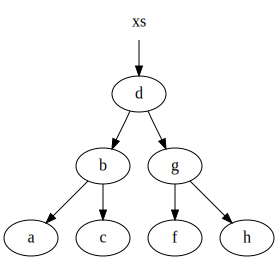
\includegraphics[scale=0.16]{tree.epsi}
  \caption{A Binary Tree}
  \label{tree}
\end{figure}


\begin{figure}[ht]
  \begin{adjustwidth}{-2em}{}
  \begin{minipage}[b]{0.5\linewidth}
    \centering
    \includegraphics[scale=0.6]{desup.epsi}
    \caption{Destructive Update}
    \label{desup}
  \end{minipage}
  \hspace{0.6cm}
  \begin{minipage}[b]{0.5\linewidth}
    \centering
    \includegraphics[scale=0.6]{nondes.epsi}
    \caption{Nondestructive Update}
    \label{nondesup}
  \end{minipage}
  \end{adjustwidth}
\end{figure}

The property of persistence makes purely functional data structures the
right choice for the applications that need to maintain multiple
versions of the data structure especially to support programming in
functional style and immutability in these data structures makes it
easier to reason about the parallelism in programs. Operations on purely
functional data structure can be performed in parallel because there are
no side effects changing the data structure.

%The applications which need to maintain multiple versions of the data
%structure 

%\begin{figure} [htb]
%  \centering
%  \includegraphics[scale=0.7]{desup.epsi}
%  \includegraphics[scale=0.7]{nondes.epsi}
%  \caption{Destructive Update}
%  \label{desup}
%\end{figure}

%\begin{figure} [htb]
%  \centering
%  \includegraphics[scale=0.25]{per3.png}
%  \caption{Nondestructive Update}
%  \label{nondesup}
%\end{figure}

%\begin{center}
%\end{center}

%\PSbox{out.ps hscale=25 vscale=25}{0.25in}{0.25in}

\section{Choice of Data Structures}

The chosen data structures provide a wide variety of performance
characteristics and APIs. They include data structures designed for
particular use cases and those that are only performant for certain
operations. These include a variety of single and double-ended queues
(otherwise known as deques), variants of heaps and sets, red-black
trees, treaps, tries and hash lists. Implementing a wide variety of data
structures with the same API allows studying the practical performance
characteristics of each variant, since different variants provide widely
varying running times for specific operations.

%Functional data structures chosen for implementation include functional
%data structures with different performance characteristics, that provide
%different APIs and data structures in which only certain operations are
%performant and hence are suitable only for certain applications. The
%data structures implemented include variants of FIFO queues, variants of
%double ended queues aka deques, variants of lists, variants of heaps,
%variants of sets, red-black tree, treap, tries, and hash list. All the
%variants of the same kind data structure were implemented to study the
%practical performance characteristics of each variant as each variant
%provides different algorithmic running times for its operations.

Another factor influencing the variety of data structures is Typed
Racket. By choosing a wide variety of data structures, each with its own
type invariants and type system requirements, Typed Racket's type system
is exercised and validated in many different ways.

\section{Data Structure Interfaces}

%The library developed to support this thesis consists of more than 25
%distinct data structures.

All the data structures in the library are polymorphic in their element
type and provide utility functions such as \scheme|map|, \scheme|fold|
and \scheme|filter| as well as basic API operations. Each of the queue
implementations share a common API, and similarly for deques, heaps and
other data structures. The following subsections describe the basic
interface of the each category of data structure.

\subsection{Queue Interface}
Queues are First-In-First-Out (FIFO) data structures. All the queue
implementations in the library use the type \scheme|(Queue alpha)|,
where \scheme|alpha| is the polymorphic type variable. Each queue data
structure shares the following common interface:

\begin{file}{Queue Interface}
\begin{schemedisplay}
  ;; Constructs a queue of type \scheme|(Queue alpha)|.
  (: queue : (All (alpha) alpha * -> (Queue alpha))


  ;; Checks if the given queue is empty
  (: empty? : (All (alpha) (Queue alpha) -> Boolean))
  

  ;; Returns the first element of the given queue.
  (: head : (All (alpha) (Queue alpha) -> alpha)


  ;; Returns the tail of the given queue, i.e. a queue without the
  ;; first element of the given queue.
  (: tail : (All (alpha) (Queue alpha) -> (Queue alpha))


  ;; Inserts the given element into the given queue.
  (: enqueue : (All (alpha) alpha (Queue alpha) -> (Queue alpha)))

\end{schemedisplay}
\end{file}

%\vspace{4 mm}

%\scheme|empty?| : \scheme|(All (alpha) (Queue alpha) -> Boolean)|
%\noindent
%\\
%Checks if the given queue is empty.
% 
%\vspace{4 mm}
% 
%\scheme|queue->list| : \scheme|(All (alpha) (Queue alpha) -> (Listof alpha))|
%\noindent
%\\
%Returns a list of all the elements in the given queue. 

%----------------------------------------------------------------


\subsection{Interface for Deque}
Double ended queues are also known as deques. Elements can be inserted
and removed from either end of a deque. The following basic interface
are provided by deque data structure and they have the type
\scheme|(Deque alpha)|:

\begin{file}{Deque Interface}
  \begin{schemedisplay}
    ;; Constructs a deque of type \scheme|(Deque alpha)|.
    (: deque : (All (alpha) alpha * -> (Deque alpha)))

    ;; Checks if the given deque is empty
    (: empty? : (All (alpha) ((Deque alpha) -> Boolean)))

    ;; Returns the first element of the given deque.
    (: head : (All (alpha) (Deque alpha) -> alpha))


    ;; Returns the last element of the given deque.
    (: last : (All (alpha) (Deque alpha) -> alpha))


    ;; Returns the tail of the given deque, i.e. a deque without the first
    ;; element of the given deque.
    (: tail : (All (alpha) (Deque alpha) -> (Deque alpha)))


    ;; Returns a deque without the last element of the given deque.
    (: init : (All (alpha) (Deque alpha) -> (Deque alpha)))


    ;; Inserts the given element to the rear of the given deque.
    (: enqueue : (All (alpha) alpha (Deque alpha) -> (Deque alpha)))


    ;; Inserts the given element to the front of the given deque.
    (: enqueue-front : (All (alpha) alpha (Deque alpha) -> (Deque alpha)))

  \end{schemedisplay}
\end{file}
  
%\vspace{4 mm}
% 
%\scheme|empty?| : \scheme|(All (alpha) (Deque alpha) -> Boolean)|
%\noindent
%\\
%Checks if the given deque is empty.
% 
%\vspace{4 mm}
% 
%\scheme|deque->list| : \scheme|(All (alpha) (Deque alpha) -> (Listof alpha))|
%\noindent
%\\
%Returns a list of all the elements in the given deque.


%\clearpage
\subsection{Heap Interface}

Heaps are tree-based data structures that satisfy two additional
constraints:

\begin{description}
\item[Shape] All its levels of the tree must be full
  except the last level where only rightmost leaves may be missing.
\item[Parental Dominance] The key at each node of the tree
  must greater than or equal (max-heap) OR less than or equal (min-heap)
  to the keys of its children.
%  A tree satisfying this property is said to be \emph{heap-ordered}.
\end{description}
\noindent
All the heaps have the type \scheme|(Heap alpha)|:

\begin{file}{Heap Interface}
  \begin{schemedisplay}

    ;; Constructs a heap with the given elements and 
    ;; \scheme|(alpha alpha -> Boolean)| as its comparison function.
    (: heap : (All (alpha) (alpha alpha -> Boolean) alpha * -> (Heap alpha)))


    ;; Checks if the given heap is empty.
    (: empty? : (All (A) ((Heap A) -> Boolean)))

    
    ;; Inserts the given element into the given heap.
    (: insert : (All (alpha) alpha (Heap alpha) -> (Heap alpha)))


    ;; Returns the min or the max element of the given heap.
    (: find-min/max : (All (alpha) (Heap alpha) -> alpha))


    ;; Deletes the min or the max element of the given heap.
    (: delete-min/max : (All (alpha) (Heap alpha) -> (Heap alpha)))

  \end{schemedisplay}
\end{file}
%\vspace{4 mm}
% 
%\scheme|sorted-list| : \scheme|(All (alpha) (Heap alpha) -> (Listof alpha))|
%\noindent
%\\
%Creates a sorted list of elements out of the elements from the given
%heap sorted with the comparison function of the heap.


\subsection{List Interface}

Alternatives to the Racket's built-in lists. They have the type
\scheme|(List alpha)|\footnote{Typed Racket also provides a built-in
type \scheme|(List alpha)|. The two types can be disambiguated using
Racket's module system.} and provide the following functions:


\begin{file}{List Interface}
  \begin{schemedisplay}
    ;; Constructs a list with the given elements.
    (: list : (All (alpha) alpha * -> (List alpha)))

    ;; Checks if the given list is empty.
    (: empty? : (All (alpha) ((List alpha) -> Boolean)))


    ;; Adds the given element to the front of the given list.
    (: cons : (All (alpha) alpha (List alpha) -> (List alpha)))


    ;; Returns the first element of the given list.
    (: first : (All (alpha) (List alpha) -> alpha))


    ;; Returns the list without the first element of the given list.
    (: rest : (All (alpha) (List alpha) -> (List alpha)))

  \end{schemedisplay}
\end{file}

\subsection*{Random Access List}
Random Access Lists are lists with efficient array-like random access
operations. These include \scheme|list-ref| and \scheme|list-set| (a
functional analogue of \scheme|vector-set!|). Random Access Lists
extend the basic list interface with the following operations:

\begin{file}{RAList Interface}
  \begin{schemedisplay}

    ;; Returns the element at a given location in the list.
    (: list-ref : (All (alpha) Natural (List alpha) -> (List alpha)))


    ;; Updates the element at a given location in the list with a new element.
    (: list-set : (All (alpha) Natural (List alpha) alpha -> (List alpha)))

  \end{schemedisplay}
\end{file}

\subsection*{Catenable List}
Catenable Lists are a list data structure with an efficient append
operation:

\begin{file}{Catenable List Interface}
  \begin{schemedisplay}

    ;; Appends several lists together.
    (: append : (All (alpha) (List alpha) * -> (List alpha))

    
    ;; Inserts a given element to the rear end of the list.
    (: cons-to-end : (All (alpha) alpha (List alpha) -> (List alpha)))

  \end{schemedisplay}
\end{file}
%\vspace{4 mm}



%\vspace{4 mm}
% 
%\scheme|length| : \scheme|(All (alpha) (List alpha) -> Natural)|
%\noindent
%\\
%Returns the length of the given list.


 

%\subsection{Interface for Sets}


%Other data structures include treaps, red-black
%trees, streams and tries. In this chapter, I describe the structure,
%contents of the library, report their performance and compare them with
%imperative data structures.

\section{Data Structure Implementation}

This section describes the theory and performance characteristics of
each data structure in the library.
%and shows example uses of each data structure.

\subsection{Queue Implementations}

\subsection*{Banker's Queue}

Banker's Queues \citep{oka} use a method of amortization known as the
banker's method. Banker's Queues combine lazy evaluation and memoization
to obtain \emph{O}(1) amortized running times for the \scheme|head|,
\scheme|tail| and \scheme|enqueue| operations. The implementation uses
lazy lists to achieve lazy evaluation. The basic structure of Banker's
Queue is similar to the Batched Queue implementation from
Figure~\ref{fig:queueds}. The difference between the two definitions is
that Banker's Queue uses streams as described in Section~\ref{stream}
instead of lists and maintains the invariant \scheme|lenf leq lenr|.

\begin{datastructure}
\begin{schemedisplay}
  langtr

  (struct: (alpha) Queue
    ([front : (Stream alpha)]
     [lenf  : Natural]
     [rear  : (Stream alpha)]
     [lenr  : Natural]))

\end{schemedisplay}
\end{datastructure}

%Banker's Queues provide a amortized running time of \emph{O}(1) .

\subsection*{Physicist's Queue}
\label{phy}
Physicist's Queue \citep{oka} uses a method of amortization called the
physicist's method. The Physicist's Queue also uses lazy evaluation and
memoization to achieve improved amortized running times for its
operations. The only drawback of the physicist's method is that it is
much more complicated than the banker's method.

Unlike Banker's Queues, Physicist's Queues use suspended lists of type
\scheme|(Promise (Listof alpha))| for front instead of streams. Streams
are similar to \scheme|cons|-lists except that every cell in a stream is
delayed. In contrast, suspended lists wrap ordinary \scheme|cons|-lists
in a single delay. The rear is an ordinary list and is not suspended.

The lengths of the lists are explicitly tracked and guaranteed that the
front list is always at least as long as the rear list. Since the front
list is delayed, its first element cannot be accessed without executing
the entire suspension. So, a working copy of a prefix of the front list
is also maintained. This working copy is represented as an ordinary list
for efficient access, and is non-empty whenever the front list is
non-empty. The following box shows the underlying structure of
Physicist's Queue.

\begin{datastructure}
\begin{schemedisplay}
  langtr

  (struct: (alpha) Queue
    ([pref  : (Listof alpha)]
     [front : (Promise (Listof alpha))]
     [lenf  : Natural]
     [rear  : (Listof alpha)]
     [lenr  : Natural]))

\end{schemedisplay}
\end{datastructure}

The Physicist's Queue provides an amortized running time of \emph{O}(1)
for the operations \scheme|head|, \scheme|tail| and
\scheme|enqueue|. The implementation of Physicist's Queue is slightly
complicated than Banker's Queue though they have the same amortized
running times.

\subsection*{Real-Time Queue}
Real-Time Queues eliminate the amortization of the Banker's and
Physicist's Queues to produce a queue with excellent worst-case as well
as amortized running times. Real-Time Queues employ lazy evaluation and
a technique called \emph{scheduling} \citep{oka} where lazy components
are forced systematically so that no suspension takes more than constant
time to execute, assuring good asymptotic worst-case running time for
the operations on the data structure. The structure of Real-Time Queues
differs from Banker's Queues in three ways. First, Real-Time Queues
maintain an extra field of type \scheme|(Stream alpha)| called a
\scheme|schedule|, which determines when \scheme|front| is
forced. Second, Real-Time Queues does not maintain length fields as the
information is available in \scheme|schedule|. And third, \scheme|rear|
is a list and not a stream.

\begin{datastructure}
\begin{schemedisplay}
  langtr
  
  (struct: (alpha) Queue
    ([front      : (Stream alpha)]
     [rear       : (Listof alpha)]
     [schedule : (Stream alpha)]))
\end{schemedisplay}
\end{datastructure}

Unlike Physicist's Queues and Banker's Queues which have a amortized
running times, Real-Time Queues have an \emph{O}(1) worst-case running
time for the operations \scheme|head|, \scheme|tail| and
\scheme|enqueue|.


\subsection*{Implicit Queue}
Implicit Queues implement a queue data structure via \emph{implicit
recursive slowdown} \citep{oka}. Implicit recursive slowdown combines
laziness with a technique called \emph{recursive slowdown} introduced by
\cite{kaplan-tarjan}. This technique is simpler than pure recursive
slow-down, but with the disadvantage of amortized rather than worst-case
bounds on the running time. Similar to Physicist's Queues and Banker's
Queues and unlike Real-Time Queues, Implicit Queues provide an amortized
running time of \emph{O}(1) for the operations \scheme|head|,
\scheme|tail| and \scheme|enqueue|.


\subsection*{Bootstrapped Queue}
The technique of \emph{bootstrapping} is applicable to problems whose
solutions require solutions to simpler instances of the same
problem. Bootstrapped Queues use \emph{structural decomposition}
\citep{oka}.  In structural decomposition, an implementation that can
handle data up to a certain bounded size is used to implement a data
structure that can handle data of unbounded size. Bootstrapped Queues
give a worst-case running time of \emph{O}(1) for the operation
\scheme|head| and \emph{O}(log*~n) for \scheme|tail| and \scheme|enqueue|.
Any queue implementation can be used for bootstrapping. For performance
reasons, my implementation of Bootstrapped Queue uses Physicist's Queue
for bootstrapping.

%\footnote[1]{\emph{log*n} is at most 5 for all feasible queue lengths.}

\subsection*{Hood-Melville Queue}
Hood-Melville Queues \citep{hood-mel} resemble Real-Time Queues in many
ways. Both Real-Time and Hood-Melville Queues maintain two lists front
and rear and incrementally rotate the elements from rear list to front
list when the rear list becomes longer than the front list. The way the
elements are rotated is different. Hood-Melville Queues use a more
complex technique, called \emph{global rebuilding}. In global
rebuilding, reversing of the rear list is done incrementally, a few
steps of reversing per normal operation on the data
structure. Hood-Melville Queues have worst-case running times of
\emph{O}(1) for the operations \scheme|head|, \scheme|tail| and
\scheme|enqueue|.

\subsection{Deque Implementations}

\subsection*{Banker's Deque}
Banker's Deques \cite{oka} are double-ended queues with amortized
running times. They use the banker's method. The structure of Banker's
Deque is similar to the structure of Banker's Queue, using streams and
employing the same techniques used in Banker's Queues to achieve
amortized running times of \emph{O}(1) for the operations \scheme|head|,
\scheme|tail|, \scheme|last|, \scheme|init|, \scheme|enqueue-front| and
\scheme|enqueue|.


\subsection*{Implicit Deque}
The techniques used by Implicit Deques are same as that used in Implicit
Queues i.e., implicit recursive slowdown \citep{oka}. Implicit Deques
provide \emph{O}(1) amortized running times for the operations
\scheme|head|, \scheme|tail|, \scheme|last|, \scheme|init|,
\scheme|enqueue-front| and \scheme|enqueue|.


\subsection*{Real-Time Deque}
Real-Time Deques \citep{oka} eliminate the amortization in the Banker's
Deque to produce deques with good worst-case behavior. The Real-Time
Deques employ the same techniques employed by the Real-Time Queues to
provide worst-case running time of \emph{O}(1) for the operations
\scheme|head|, \scheme|tail|, \scheme|last|, \scheme|init|,
\scheme|enqueue-front| and \scheme|enqueue|.

\subsection{Heap Implementations}

\subsection*{Binomial Heap}
A Binomial Heap \citep{vuillemin, brown} is a heap-ordered binomial
tree. Binomial trees maintains a natural number called its
\emph{rank}. The tree structure is defined as follows:
\begin{itemize}
  \item{A Binomial Tree with rank 0 is a leaf with one element.}

  \item{A Binomial Tree with rank \scheme|r + 1| is composed of two
  trees of rank \scheme|r|.}
\end{itemize}

Binomial Heaps support a fast \scheme|merge| operation using the special
tree structure. Data~Structure~\ref{ds:5} the underlying structure of
Binomial Heaps in Typed Racket.

\begin{datastructure}
  \begin{schemedisplay}

    (struct: (alpha) Node
      ([rank : Natural]
       [elem : alpha]
       [trees : (Listof (Node alpha))]))

    (struct: (alpha) Heap
      ([compare : (alpha alpha -> Boolean)]
       [trees       : (Listof (Node alpha))]))
  \end{schemedisplay}
  \label{ds:5}
\end{datastructure}

\noindent
Binomial Heaps provide a worst-case running time of \emph{O}(log~n) for
the operations \scheme|insert|, \scheme|find-min/max| and
\scheme|delete-min/max|.

\subsection*{Leftist Heap}
Leftist Heaps \citep{crane} are heap-ordered binary trees that satisfy
the \emph{leftist property}.  Each node in the tree is assigned a value
called a \emph{rank}.  The rank represents the length of its rightmost
path from the node in question to the nearest leaf. The leftist property
requires that the right descendant of each node has a lower rank than
the node itself. As a consequence of the leftist property, the right
spine of any node is always the shortest path to a leaf
node. Data~Structure~\ref{ds:6} shows the structure of Leftist Heaps in
Typed Racket.% is:% defined as follows.

\begin{datastructure}
  \begin{schemedisplay}

    (struct: (alpha) Node
      ([rank : Natural]
       [elem : alpha]
       [left   : (Tree alpha)]
       [right : (Tree alpha)]))

    (define-type (Tree alpha) (U Null (Node alpha)))

    (struct: (alpha) Heap
      ([compare : (alpha alpha -> Boolean)]
       [tree        : (Tree alpha)]))

  \end{schemedisplay}
  \label{ds:6}
\end{datastructure}

\noindent
The Leftist Heaps provide a worst-case running time of \emph{O}(log~n)
for the operations \scheme|insert|, \scheme|delete-min/max|,
\scheme|merge| and a worst-case running time of \emph{O}(1) for
\scheme|find-min/max|.

\subsection*{Pairing Heap}
Pairing Heaps \citep{pairing} are a type of heap that simultaneously
have a simple implementation and extremely good amortized performance in
practice. Unfortunately pairing heaps do not cope well with persistence
and hence can be used only in applications that do not take advantage
of persistence.
%However, it has proved very difficult to come up with exact
%asymptotic running time for some operations on Pairing Heaps.
Pairing Heaps are heap-ordered multiway trees represented either as a
empty heap or a pair of an element and a list of pairing
heaps. Data~Structure~\ref{ds:7} shows the structure of Pairing Heaps
in Typed Racket.% is:

\begin{datastructure}
  \begin{schemedisplay}

    (struct: (alpha) Node
      ([elem : alpha]
       [trees : (Listof (Tree alpha))]))

    (define-type (Tree alpha) (U Null (Node alpha)))

    (struct: (alpha) Heap
      ([compare : (alpha alpha -> Boolean)]
       [heap       : (Tree alpha)]))

  \end{schemedisplay}
  \label{ds:7}
\end{datastructure}

\noindent
Pairing Heaps provide a worst-case running time of \emph{O}(1) for the
operations \scheme|insert|, \scheme|find-min/max| and \scheme|merge|,
and an amortized running time of \emph{O}(log~n) for
\scheme|delete-min/max|.

\subsection*{Splay Heap}
Splay Heaps \citep{sla} are similar to balanced binary search trees.
Data~Structure~\ref{ds:8} shows the structure of Splay Heaps in Typed
Racket.
% is:

\begin{datastructure}
  \begin{schemedisplay}

    (struct: (alpha) Node
      ([element : alpha]
       [left        : (Tree alpha)]
       [right      : (Tree alpha)]))

    (define-type (Tree alpha) (U Null (Node alpha)))

    (struct: (alpha) Heap 
      ([compare : (alpha alpha -> Boolean)]
       [heap       : (Tree alpha)]))

  \end{schemedisplay}
  \label{ds:8}
\end{datastructure}

\noindent
The difference between a Splay Heap and a balanced binary search tree is
that Splay Heaps do not maintain explicit balance information. Instead,
every operation on a splay heap restructures the tree with
transformations that increase the balance. Because of the restructuring
on every operation, the worst-case running time of all operations is
\emph{O}(n). However, the amortized running time of the operations
\scheme|insert|, \scheme|find-min/max|, \scheme|delete-min/max| and
\scheme|merge| is \emph{O}(log~n).

\subsection*{Skew Binomial Heap}
Skew Binomial Heaps are similar to Binomial Heaps but with a hybrid
numerical representation for heaps that is based on the \emph{skew
  binary numbers} \citep{skew}. The skew binary number representation is
used since incrementing skew binary numbers is quick and simple. Since
the skew binary numbers have a complicated addition, the \scheme|merge|
operation is based on the ordinary binary numbers itself. Skew Binomial
Heaps provide a worst-case running time of \emph{O}(log~n) for the
operations \scheme|find-min/max|, \scheme|delete-min/max| and
\scheme|merge|, and a worst-case running time of \emph{O}(1) for the
\scheme|insert| operation.

\subsection*{Lazy Pairing Heap}
Lazy Pairing Heaps \citep{oka} are similar to pairing heaps, except that
Lazy Pairing Heaps use lazy evaluation.  Lazy evaluation is used in this
data structure so that the Pairing Heap can cope with persistence
efficiently. Analysis of Lazy Pairing Heaps to obtain exact asymptotic
running times is difficult, as it is for Pairing Heaps. Lazy Pairing
Heaps provide a worst-case running time of \emph{O}(1) for the
operations \scheme|insert|, \scheme|find-min/max|, and \scheme|merge|,
and an amortized running time of \emph{O}(log~n) for the
\scheme|delete-min/max| operation.

\subsection*{Bootstrapped Heap}
Bootstrapped Heaps \citep{oka} use a technique of bootstrapping called
\emph{structural abstraction}, where one data structure abstracts over a
less efficient data structure to get better running times.  Bootstrapped
Heaps provide a worst-case running time of \emph{O}(1) for the
\scheme|insert|, \scheme|find-min/max| and \scheme|merge| operations and
a worst-case running time of \emph{O}(log~n) for \scheme|delete-min/max|
operation. Any heap implementation can be used for bootstrapping. For
practical reasons, my implementation of Bootstrapped Heap abstracts over
Skew Binomial Heaps.

%Due The implementation of Bootstrapped Heap
%abstracts over Skew Binomial Heaps though any other heap implementation
%could be used.

\subsection{List Implementations}
%\subsection*{Random Access List}
%Random Access Lists are lists with efficient array-like random access
%operations. These include \scheme|list-ref| and \scheme|list-set| (a
%functional analogue of \scheme|vector-set!|). Random Access Lists extend
%the basic list interface with \scheme|list-ref| and \scheme|list-set|
%operations.
%\begin{itemlist}
%  \item{\scheme|list-ref : (All (alpha) (List alpha) Integer → alpha)|
%         Returns the element at a given location in the list.}
%  \item{\scheme|list-set : (All (alpha) (List alpha) Integer alpha → (List alpha))|
%    Updates the element at a given location in the list with a new element.}
%)

%\scheme|list-ref : (All (alpha) Natural (List alpha) -> (List alpha))|
%\noindent
%\\
%Returns the element at a given location in the list.
% 
%\vspace{4 mm}
% 
%\scheme|list-set : (All (alpha) Natural (List alpha) alpha -> (List alpha))|
%\noindent
%\\
%Updates the element at a given location in the list with a new element

\subsection*{Binary Random Access List}
Binary Random Access Lists abstract the similarities between
representations of the numbers and lists to derive a representation of
list structure. The Binary Random Access List representation abstracts
over the binary numerical representation \citep{oka} to achieve a
worst-case running time of \emph{O}(log~n) for its random-access
operations \scheme|list-ref| and
\scheme|list-set|. Data~Structure~\ref{ds:9} shows the structure of he
structure of Binary Random Access Lists in Typed Racket.

\begin{datastructure}
  \begin{schemedisplay}

    (struct: (alpha) Leaf ([first : alpha]))

    (struct: (alpha) Node 
      ([first  : alpha]
       [left    : (Tree alpha)] 
       [right : (Tree alpha)]))

    (define-type (Tree alpha) (U (Leaf alpha) (Node alpha)))

    (struct: (alpha) Root 
      ([size  : Integer]
       [first : (Tree alpha)]
       [rest  : (List alpha)]))

    (define-type (List alpha) (U Null (Root alpha)))

  \end{schemedisplay}
  \label{ds:9}
\end{datastructure}

\noindent
Binary Random Access Lists provide a worst-case running time of
\emph{O}(log~n) for the operations \scheme|cons|, \scheme|first| and
\scheme|rest| contrary to Typed Racket's built-in list's worst-case
running time of \emph{O}(1) for the same operations.

\subsection*{Skew Binary Random Access List}
Skew Binary Random Access Lists are similar to Binary Random Access
Lists, but use the skew binary number representation, improving the
running times of some operations. Unlike Binary Random Access Lists,
that have worst-case running time of \emph{O}(log~n), Skew Binary Random
Access Lists provide worst-case running time of \emph{O}(1) for the
operations \scheme|cons|, \scheme|head| and \scheme|tail|. And like
Binary Random Access Lists, Skew Binary Random Access Lists also provide
worst-case running time of \emph{O}(log~n) for \scheme|list-ref| and
\scheme|list-set| operations.

\subsection*{VList}
VLists \citep{bagwell-lists} resemble normal cons lists but provide
efficient versions of many operations that are much slower on standard
lists. They combine the extensibility of linked lists with the fast
random access capability of arrays. Data~Structure~\ref{ds:10} shows the
structure of VLists in Typed Racket. The \scheme|elements| field in the
\scheme|Base| in Data~Structure~\ref{ds:10} is a random access list.
%, along with many other operations,
%some of them are given below.


%\scheme|last| : \scheme|(All (alpha) (List alpha) -> alpha)| \\
%Returns the last element of the given list.
%\vspace{4 mm}
% 
%\scheme|list-ref| : \scheme|(All (alpha) (List alpha) Integer -> alpha)| \\
%Gets the element at the given index in the list.

\begin{datastructure}
  \begin{schemedisplay}
    langtr

    (struct: (alpha) Base
      ([previous : (Block alpha)]
       [elements : (List alpha)]))

    (define-type (Block alpha) (U Null (Base alpha)))

    (struct: (alpha) VList
      ([offset : Integer]
       [base   : (Base alpha)]
       [size    : Integer]))

  \end{schemedisplay}
  \label{ds:10}
\end{datastructure}

\noindent
VLists provide worst-case running times of \emph{O}(1) for the
operations \scheme|cons|, \scheme|head| and \scheme|tail|,
\scheme|list-ref| and \scheme|list-set| operations. This VList
implementation is built internally on Skew Binary Random Access
Lists. VLists provide the standard Random Access List API operations.

\subsection*{Catenable List}
%@subsection[#:tag "catenable"]{Catenable List}
Catenable Lists \citep{catenable} are a list data structure with an
efficient append operation, achieved using the bootstrapping technique
of \emph{structural abstraction}. Catenable Lists are abstracted over
Bootstrapped Queue. They have an amortized running time of \emph{O}(1)
for the basic list operations and for the operations
\scheme|cons-to-end| and \scheme|append|.
%It has the type \scheme|(List alpha)|.

\subsection*{Streams}
\label{stream}
Streams \citep{oka} are also known as lazy lists. They are similar to
ordinary lists and provide a similar API. Stream API provides
\scheme|stream|, \scheme|stream-car|, \scheme|stream-cdr| and
\scheme|stream-cons| which are similar to \scheme|list|, \scheme|first|,
\scheme|rest| and \scheme|cons| from the list interface
respectively. Along with these basic functions, Stream API also provide
some utility functions. Many data structures implemented in this library
use Streams to achieve lazy evaluation. Streams do not change the
asymptotic performance of any list operations, but introduce overhead at
each suspension. And forcing a suspension takes no more than \emph{O}(1)
and hence \scheme|stream-car|, \scheme|stream-cdr| and
\scheme|stream-cons| have a running time of \emph{O}(1). Since streams
have distinct evaluation behavior, they are given a distinct type,
\scheme|(Stream alpha)|.


\subsection{Other Data Structures}
\subsection*{Hash Lists}
Hash Lists \citep{bagwell-lists} are similar to association lists, and
are implemented using a modified VList structure. The modified VList
contains two components: the data and the hash table. Both components
grow as the hash list grows. The running time for Hash Lists operations
such as \scheme|insert|, \scheme|delete|, and \scheme|lookup| are close
to those for standard chained hash tables.

\subsection*{Tries}
A Trie (also known as a Digital Search Tree) \citep{oka} is a data
structure that takes advantage of the structure of aggregate types to
achieve good running times for its operations. Our implementation
provides Tries in which the keys are lists of the element type; this is
sufficient for representing many aggregate data structures. In our
implementation, each trie is a multiway tree with each node of the
multiway tree carrying data of base element type.  Tries provide
\scheme|lookup| and \scheme|insert| operations with better asymptotic
running times than hash tables.

\subsection*{Red-Black Tree}
Red-Black Trees \citep{red-black} are a classic data structure,
consisting of a binary search trees in which every node is colored
either red or black, according to the following two balance invariants:

\begin{itemize}
\item{no red node has a red child, and}
\item{every path from root to an empty node has the same number of black
  nodes.}
\end{itemize}
  
The two invariants together guarantee that the longest possible path
with alternating black and red nodes, is no more then twice as long as
the shortest possible path, with black nodes only. This property helps
achieve good running times for the tree operations. This implementation
is based on \citet{oka-red-black}. Data~Structure~\ref{ds:11} shows the
structure of Red-Black Trees in Typed Racket.

\begin{datastructure}
  \begin{schemedisplay}
    langtr

    (define-type Color (U 'red 'black))
     
    (struct: (alpha) RedBlackNode
      ([color     : Color]
       [element : alpha]
       [left        : (Tree alpha)]
       [right      : (Tree alpha)]))
     
    (define-type (Tree alpha) (U Null (RedBlackNode alpha)))
     
    (struct: (alpha) RedBlackTree
      ([compare : (alpha alpha -> Boolean)]
       [tree        : (Tree alpha)]))

  \end{schemedisplay}
  \label{ds:11}
\end{datastructure}

The operations \scheme|member?|, \scheme|insert| and \scheme|delete|,
which respectively check membership, insert and delete elements from the
tree, have worst-case running time of \emph{O}(log~n). Red-Black Trees
have the type \scheme|(RedBlackTree alpha)|.


\subsection*{Treap}
Treaps \citep{treap} are binary search trees in which each node has both
a search key and a priority. Its keys are sorted in-order and the
priority of each node is lower than the priorities of its
children. Because of these properties, a treap is a binary search tree
for the keys and a heap for its priorities. Assigning random priorities
to the nodes of the treap results in better balance in the treap. Hence
treaps are also known as randomized binary search
trees. Data~Structure~\ref{ds:12} shows the underlying structure of
Treaps in Typed Racket.


\begin{datastructure}
  \begin{schemedisplay}
    langtr

    (struct: (alpha) Node
             ([element : alpha]
              [left        : (Tree alpha)]
              [right      : (Tree alpha)]
              [priority  : Real]))

    (define-type (Tree alpha) (U Null (Node alpha)))

    (struct: (alpha) Treap
             ([compare : (alpha alpha -> Boolean)]
              [tree        : (Tree alpha)]
              [size        : Integer]))

  \end{schemedisplay}
  \label{ds:12}
\end{datastructure}
Treaps implement a worst case running time of \emph{O}(log~n) for the
operations \scheme|insert|, \scheme|find-min/max| and
\scheme|delete-min/max|. A Treap has the type \scheme|(Treap alpha)|.

%Following are the functions implemented by the Red-Black Tree data structure
% 
%@(itemlist 
%  @item{@italic{redblacktree} : 
%         @racketblock[(∀ (A) ((A A → Boolean) A * → 
%                                          (RedBlackTree A)))| 
%         The Red-Black Tree constructor function. Constructs 
%         a red-black tree from the given elements and the
%         comparison function.}
%  @item{@italic{insert} : @racketblock[(∀ (A) (A (RedBlackTree A) → 
%                                                   (RedBlackTree A)))| 
%         @para{Inserts a given element into the red-black tree.}}
%  @item{@italic{root} : \scheme|(∀ (A) ((RedBlackTree A) → A))| 
%         @para{Returns the root element of the given red-black tree.}}
%  @item{@italic{member?} : @racketblock[(∀ (A) (A (RedBlackTree A) → Boolean))| 
%         Checks if the given element is a member of the 
%         red-black tree.}
%  @item{@italic{delete} : @racketblock[(∀ (A) (A (RedBlackTree A) → 
%                                                   (RedBlackTree A)))| 
%         @para{Deletes the given element from the given red-black 
%         tree.}})

  

%\clearpage


\chapter{Performance Analysis}
\label{chap:four}
This chapter reports on my performance evaluation of the library using
micro-benchmarks. The results demonstrate the practical usefulness of
purely functional data structures. The benchmarks compare the
performance of my purely functional data structures with each other and
with simple functional implementations based on lists and with
imperative implementations already available as Racket libraries. All
the data structures are implemented in Typed Racket, with the exception
of the pre-existing imperative versions which are implemented in untyped
Racket. Data structures in untyped Racket and Typed Racket are
benchmarked in their respective languages to ensure comparability;
otherwise language boundary-crossing would impose substantial contract
overheads.

The benchmarking was done on a 2.1 GHz Intel Core 2 Duo (Linux) machine
using Racket version 5.0.2. Each benchmark was run 10 times, with times
measured by the Racket's \scheme|time| form. In the tables below, all
times are milliseconds of CPU time as reported by Racket, including garbage
collection time.% and the times mentioned are in milliseconds.


\section{Queue Performance}

\footnotetext[1]{The constructor functions \scheme|queue|, \scheme|heap|
and \scheme|list| were repeated only 100 times.}

Table~\ref{fig:queue} shows the performance of the Physicist's Queue,
Banker's Queue, Real-Time Queue and Bootstrapped Queue compared with a
naive implementation based on lists and an imperative queue from the
Racket standard library. Some functions of the imperative queue from the
Racket standard library provide contracts. In the benchmarks where these
functions are used, separate benchmarks for the implementation without
contracts has been provided. The \emph{Size} column in
Table~\ref{fig:queue} indicates the initial size of the queue and the
times are the time taken for performing each operation 100000 times on
queues of different initial sizes, averaged over 10 runs. Because the
\scheme|head| operation runs in a very short amount of time, it is
repeated 1000000 times to reduce noise in the benchmark.

Benchmark~Code~\ref{bm:3} shows the Typed Racket code used for
generating the benchmarks for the \scheme|enqueue| operation; the
untyped Racket benchmarks are run with an equivalent untyped script.

%\footnotetext[1]{The functions \scheme|head| and \scheme|find| were
%repeated 1000000 times to improve the expressiveness of the benchmarks.}


\begin{benchmark}
 \begin{schemedisplay}
   (define Size 1000)

   (: que : (Queue Integer))
   (define que (build-queue Size add1))

   (: list : (Listof Integer))
   (define list (build-list 100000 add1))

   (time (foldl enqueue que list))

 \end{schemedisplay}
 \label{bm:3}
\end{benchmark}


%Interesting performance characteristics of each Queue implementation can
%be derived from the results of the benchmarks from the

\begin{figure*}[ht]
  %\begin{center}
  \begin{adjustwidth}{-5em}{}
    \begin{threeparttable}
      \begin{tabular}{|c|c|c|c|c|c|c|c|}
        \hline
        Size & Operation & Banker's & Physicist's & Real-Time & Bootstrapped & List & Imperative \\
        \hline
        \multirow{3}{*}{1000} & \scheme|queue| & 72 & 16 & 137 & 20 & 6 & 24 \\
        \cline{2-8}
        & \scheme|head| & 55 & 45 & 85 & 40 & 30 & 55 \\
        \cline{2-8}
        & \scheme|enqueue| & 127 & 10 & 176 & 22 & 256450 & 12 \\
        \hline
        \multirow{3}{*}{10000} & \scheme|queue| & 887 & 232 & 1576 & 227 & 61 & 290 \\
        \cline{2-8}
        & \scheme|head| & 55 & 45 & 95 & 45 & 35 & 60 \\
        \cline{2-8}
        & \scheme|enqueue| & 132 & 11 & 172 & 18 & 314710 & 14 \\
        \hline
        \multirow{3}{*}{100000} & \scheme|queue| & 13192 & 3410 & 20332 & 2276 & 860 & 3590 \\
        \cline{2-8}
        & \scheme|head| & 60 & 40 & 90 & 50 & 35 & 60 \\
        \cline{2-8}
        & \scheme|tail| \tnote{$\dagger$} & 312 & 412 & 147 & 20 & 7 & 10 \\
        \cline{2-8}
        & \scheme|enqueue| & 72 & 12 & 224 & 18 & 1289370 & 14 \\
        \hline
        \multirow{3}{*}{1000000} & \scheme|queue| & 182858 & 65590 & 294310 & 53032 & 31480 & 68310 \\
        \cline{2-8}
        & \scheme|head| & 60 & 40 & 90 & 40 & 35 & 60 \\
        \cline{2-8}
        & \scheme|tail| \tnote{$\dagger$} & 1534 & 243 & 1078 & 20 & 8 & 10 \\
        \cline{2-8}
        & \scheme|enqueue| & 897 & 30 & 1218 & 20 & $\infty$ \tnote{$\ddagger$} & 16 \\
        \hline
      \end{tabular}
      \begin{tablenotes}%[para]
      \item[$\dagger$] Since 100000 (successive) \scheme|tail| (or
        \scheme|dequeue|) operations cannot be performed on 1000 and
        10000 element queue, the \scheme|tail| operation is omitted for
        these sizes.
      \item[$\ddagger$] Longer than 30 minutes.
      %\item[$\uparrow$] Imperative Queues with and without contracts have similar performance.
      \end{tablenotes}
    \end{threeparttable}
    %\end{center}
  \end{adjustwidth}
  \caption{Queue Performance: Individual Operations}
  \label{fig:queue}
  %\changetext{}{}{-4em}{}{}
\end{figure*}
%\end{adjustwidth}

%\footnotetext[2]{Since 100000 (successive) \scheme|tail| (or
%  \scheme|dequeue|) operations can not be performed on 1000 element
%  queue, we do not have running time for \scheme|tail| operation for
%  for these sizes.}


%\changetext{-5\baselineskip}{10em}{}{}{}

%\clearpage
\noindent
Table~\ref{fig:queue} suggests four observations:
\begin{enumerate}
\item{For the queue constructor \scheme|queue|, Physicist's Queues and
  Bootstrapped Queues perform slightly better than the imperative
  queues, the performance of imperative queues is better than Banker's
  Queues, and the queue implementation based on lists outperforms all
  the other implementations.}
\item{For the \scheme|head| operation, all the implementations perform
  better than Real-Time Queues. Performance of Physicist's Queues,
  Bootstrapped Queues and imperative queues are similar and slightly
  better than Banker's Queues. The queue implementation based on lists
  performs slightly better than all of these implementations.}
\item{For the \scheme|enqueue| operation, the implementation based on
  lists is extremely slow when compared to other implementations as
  expected. Physicist's Queues, Bootstrapped Queues and imperative
  queues have similar performance and perform better than Banker's Queue and
  Real-Time Queues.}
\item{For the \scheme|tail| operation, performance of imperative queues
  and the implementation based on lists are comparable and is slightly
  better than Bootstrapped Queues. All the other functional data
  structures are slower than these queue implementations.}
\end{enumerate}


\begin{figure*}
  %\begin{center}
  \begin{adjustwidth}{-3em}{}
    \begin{threeparttable}
      \begin{tabular}{|c|c|c|c|c|c|c|c|}
        \hline
        \# of Repetitions & Banker's & Physicist's & Real-Time & Bootstrapped & Imperative & Imperative\tnote{$\ddagger$} \\
        \hline
        1000000 & 2040  & 2010  & 2170  & 560  & 750  & 410  \\
        \hline
        2000000 & 5060  & 5040  & 4430  & 1120 & 1490 & 810  \\
        \hline
        3000000 & 7990  & 7880  & 7260  & 2180 & 2260 & 1190 \\
        \hline
        4000000 & 10240 & 10280 & 9230  & 2930 & 3780 & 1630 \\
        \hline
        5000000 & 13690 & 13670 & 11930 & 3670 & 4580 & 2140 \\
        \hline
      \end{tabular}
      \begin{tablenotes}
      \item[$\ddagger$] Imperative Queue implementation without contracts.
      \end{tablenotes}
    \end{threeparttable} 
    %\end{center}
  \end{adjustwidth}
  \caption{Queue Performance: Multiple Operations}
  \label{fig:loopq}
  %\changetext{}{}{-4em}{}{}
\end{figure*}

%\noindent
Table~\ref{fig:loopq} presents the results of a multiple-operation
workload micro benchmarks. The times in are for building a queue by
repeating the \scheme|enqueue| operation \scheme|N| times and then
performing \scheme|head| and \scheme|tail| on the resulting queue
\scheme|N| times with \scheme|N| taking the values 1000000, 2000000,
3000000, 4000000 and 5000000, again averaged over 10
runs. Benchmark~Code~\ref{bm:1} shows the Typed Racket code used to
benchmark functional queues in Typed Racket. Untyped benchmark code in
Racket similar to Benchmark~Code~\ref{bm:1} was used to benchmark the
imperative queue implementation.


The results of the benchmarks from the Table~\ref{fig:loopq} indicate
that the performance of Bootstrapped Queues is faster than the
imperative queue implementation with contracts and the imperative queue
implementation without contracts perform better than Bootstrapped
Queues. Real-Time Queues, Banker's Queues and Physicist's Queues are all
almost 3 times slower than imperative queues.

\begin{benchmark}
 \begin{schemedisplay}
  (: benchmark : Integer -> Integer)
  (define (benchmark N)

    (: build : Integer (Queue Integer) -> (Queue Integer))
    (define (build i que)
      (if (<= i N)
          (build (add1 i) (enqueue i que))
          que))

    (: q : (Queue Integer))
    (define q (build 0 (queue)))

    (let add-all ([sum 0] [que q])
      (if (empty? que)
          sum
          (add-all (+ sum (head que)) (tail que)))))

  (time (benchmark 1000000))
 \end{schemedisplay}
 \label{bm:1}
\end{benchmark}

According to \citet{oka} Real-Time Queues are among the fastest queue
implementations. However, the above results show that the performance of
Typed Racket implementation of Real-Time Queues is slower than the other
functional queue implementations. The performance of some operations on
Physicist's Queue is comparable to the performance of Bootstrapped and
imperative Queues. But the overall performance of Bootstrapped Queue is
better than Physicist's Queue, the imperative queue implementation with
contracts and the other functional queue implementations. The imperative
queue implementation without contracts preforms better than all the
functional queue implementations.

%\begin{adjustwidth}{}{-8em}
%\changepage{}{}{-2em}{}{}{}{}{}{}
%\begin{adjustwidth}{-8em}{}
  %\changetext{-5\baselineskip}{10em}{}{}{}



\section{Heap Performance}
Table~\ref{fig:heap} shows the performance of the Leftist Heap, Pairing
Heap, Binomial Heap and Bootstrapped Heap implementations, compared with
a simple implementation based on sorted lists, and a simple imperative
heap. The \emph{Size} column of the table indicate the initial size of
the heaps. The times in the table are time taken for performing heap
operations 100000 times on heaps with different initial sizes, averaged
over 10 runs. Again, because the \scheme|find| operation runs in a very
short amount of time, it is repeated 1000000 times to reduce noise in
the benchmark.


The performance characteristics of the heap implementations can be
derived from the results of the benchmarks from the
Table~\ref{fig:heap}.

\begin{enumerate}
\item{For the heap constructor \scheme|heap|, Pairing Heaps and the
  imperative heap implementation perform similarly for smaller sizes and
  for larger sizes imperative heaps perform better than all the
  functional heap implementations. Pairing Heaps perform better than all
  the other functional heap implementations and the heap implementation
  based on lists outperforms all other implementations.}
\item{For the \scheme|insert| operation, the heap implementation based
  on lists is extremely slow. Among other heap implementations, the
  performance of imperative heaps, Binomial Heaps and Pairing Heaps is
  almost the same and is better than the other functional heap
  implementations.}
\item{For the \scheme|find| operation, the performance of almost all the
  heap implementations is very similar, except for Binomial Heaps, which
  are slower than the other heap implementations.}
\item{For the \scheme|delete| operation, the heap implementation based
  on lists outperforms the other heap implementations. Imperative heaps
  perform better than all the functional heap implementations. Among
  functional heaps, Leftist Heaps perform slightly better than Binomial
  and Pairing Heaps.}
\end{enumerate}

\begin{figure*}
  %\begin{center}
  \begin{adjustwidth}{-3em}{}
    \begin{threeparttable}
    \begin{tabular}{|c|c|c|c|c|c|c|c|}
      \hline
      Size & Operation & Binomial & Leftist & Pairing & Bootstrapped & List & Imperative \\
      \hline
      \multirow{3}{*}{1000} & \scheme|heap| & 45 & 192 & 30 & 122 & 9 & 30 \\
      \cline{2-8}
      & \scheme|insert| & 36 & 372 & 24 & 218 & 323874 & 20 \\
      \cline{2-8}
      & \scheme|find| & 480 & 40 & 40 & 45 & 35 & 40 \\
      \cline{2-8}
      \hline
      \multirow{3}{*}{10000} & \scheme|heap| & 422 & 2730 & 260 & 1283 & 76 & 360 \\
      \cline{2-8}
      & \scheme|insert| & 34 & 358 & 28 & 224 & 409051 & 24 \\
      \cline{2-8}
      & \scheme|find| & 430 & 40 & 45 & 45 & 35 & 40 \\
      \cline{2-8}
      \hline
      \multirow{3}{*}{100000} & \scheme|heap| & 6310 & 40580 & 4240 & 24418 & 1010 & 3490 \\
      \cline{2-8}
      & \scheme|insert| & 33 & 434 & 30 & 198 & 1087545 & 30 \\
      \cline{2-8}
      & \scheme|find| & 480 & 40 & 45 & 40 & 40 & 45 \\
      \cline{2-8}
      & \scheme|delete| \tnote{$\dagger$} & 986 & 528 & 462 & 1946 & 7 & 180 \\
      \cline{2-8}
      \hline
      \multirow{3}{*}{1000000} & \scheme|heap| & 109380 & 471588 & 80210 & 293788 & 11140 & 43010 \\
      \cline{2-8}
      & \scheme|insert| & 32 & 438 & 28 & 218 & $\infty$  \tnote{$\ddagger$} & 140 \\
      \cline{2-8}
      & \scheme|find| & 590 & 45 & 40 & 45 & 40 & 45 \\
      \cline{2-8}
      & \scheme|delete| \tnote{$\dagger$} & 1488 & 976 & 1489 & 3063 & 8 & 280 \\
      \cline{2-8}
      \hline
    \end{tabular}
    \begin{tablenotes}%[para]
      \item[$\dagger$] Since 100000 (successive) \scheme|delete| operations
        cannot be performed on 1000 and 10000 element heap, running time
        for \scheme|delete| operation for these sizes are not available.
      \item[$\ddagger$] Takes longer than 30 minutes.
    \end{tablenotes}
    \end{threeparttable}
  %\end{center}
    \end{adjustwidth}
  \caption{Heap Performance: Individual Operations}
  \label{fig:heap}
\end{figure*}

The times in Table~\ref{fig:heap1} are the times taken for building a
heap by repeating the \scheme|insert| operation \scheme|N| times and
then performing \scheme|find-min/max| and \scheme|delete-min/max| on the
resulting queue \scheme|N| times, with \scheme|N| taking the values
100000, 200000, 300000, 400000 and 500000. Benchmark~Code~\ref{bm:2}
shows the Typed Racket code used to benchmark functional heaps in Typed
Racket. Untyped benchmark code in Racket similar to
Benchmark~Code~\ref{bm:2} was used to benchmark the imperative heap
implementation in Racket.

The results of the benchmarks from the Table~\ref{fig:heap1} show that
Pairing Heaps perform slightly better than imperative heaps, and the
imperative heaps better than all other heap implementations.

\begin{benchmark}
 \begin{schemedisplay}
  (: benchmark : Integer -> Integer)
  (define (benchmark N)
   
    (: build : Integer (Heap Integer) -> (Heap Integer))
    (define (build i heap)
      (if (<= i N)
          (build (add1 i) (insert i heap))
          heap))

    (: init-heap : (Heap Integer))
    (define init-heap (build 0 (heap < 1)))

    (let add-all ([sum 0] [init-heap init-heap])
      (if (empty? init-heap)
          sum
          (add-all (+ sum (find-min/max init-heap))
                (delete-min/max init-heap)))))

  (time (benchmark 100000))
 \end{schemedisplay}
 \label{bm:2}
\end{benchmark}

\begin{figure*}[ht]
  \begin{adjustwidth}{0em}{}
    \begin{threeparttable}
      \begin{tabular}{|c|c|c|c|c|c|c|}
        \hline
        \# of Repetitions & Binomial & Leftist & Pairing & Bootstrapped & Imperative \\%&IBinary&IFibo\\ %& Splay \\ % & Skew Binomial
        \hline
        100000 & 290  & 620  & 120 & 320  & 240  \\%& 1060 & 810  \\ %& 160  \\ %  & 980  
        \hline%                                   \\%          
        200000 & 610  & 1330 & 320 & 660  & 480  \\%& 2270 & 1810 \\ %& 440  \\ %  & 2140 
        \hline%                                   \\%          
        300000 & 980  & 2140 & 480 & 1030 & 840  \\%& 3570 & 2760 \\ %& 730  \\ %  & 3390 
        \hline%                                   \\%          
        400000 & 1310 & 3020 & 690 & 1370 & 940  \\%& 4950 & 3690 \\ %& 1020 \\ %  & 4630 
        \hline%                                   \\%          
        500000 & 1630 & 3760 & 820 & 1660 & 1410 \\%& 6090 & 4770 \\ %& 1240 \\ %  & 4630 
        \hline
      \end{tabular}
      \caption{Heap Performance: Multiple Operations}
      \label{fig:heap1}
    \end{threeparttable} 
  \end{adjustwidth}
\end{figure*}

The results show that some functional heap implementations perform
comparable to and in some cases better than imperative heap
implementation. Among the functional heap implementations, Pairing Heaps
are fastest overall.

\section{List Performance}
Table~\ref{fig:list} shows the performance of Skew Binary Random Access
Lists and VLists compared with built-in lists. The \emph{Size} column in
the table indicate the initial size of the list. The times in the table
indicate the time taken to perform list operations 100000 times on lists
of different initial sizes. The results of the benchmark show the
performance characteristics of each list implementation.

\begin{figure*}[htb]
  \begin{adjustwidth}{+6em}{}
    \begin{threeparttable}
      \begin{tabular}{|c|c|c|c|c|}
        \hline
        Size & Operation & RAList & VList & List \\
        \hline
        \multirow{3}{*}{1000} & \scheme|list| & 24 & 51 & 2 \\
        \cline{2-5}
        & \scheme|list-ref| & 77 & 86 & 240 \\
        \cline{2-5}
        & \scheme|first| & 2 & 9 & 1 \\
        \cline{2-5}
        & \scheme|rest| & 20 & 48 & 1 \\
        \cline{2-5}
        & \scheme|last| & 178 & 40 & 520 \\
        \cline{2-5}
        \hline
        \multirow{3}{*}{10000} & \scheme|list| & 263 & 476 & 40 \\
        \cline{2-5}
        & \scheme|list-ref| & 98 & 110 & 2538 \\
        \cline{2-5}
        & \scheme|first| & 2 & 9 & 1 \\
        \cline{2-5}
        & \scheme|rest| & 9 & 28 & 1 \\
        \cline{2-5}
        & \scheme|last| & 200 & 52 & 5414 \\
        \cline{2-5}
        \hline
        \multirow{3}{*}{100000} & \scheme|list| & 2890 & 9796 & 513 \\
        \cline{2-5}
        & \scheme|list-ref| & 124 & 131 & 33187 \\
        \cline{2-5}
        & \scheme|first| & 3 & 10 & 1 \\
        \cline{2-5}
        & \scheme|rest| & 18 & 40 & 1 \\
        \cline{2-5}
        & \scheme|last| & 204 & 58 & 77217 \\
        \cline{2-5}
        \hline
        \multirow{3}{*}{1000000} & \scheme|list| & 104410 & 147510 & 4860 \\
        \cline{2-5}
        & \scheme|list-ref| & 172 & 178 & 380960 \\
        \cline{2-5}
        & \scheme|first| & 2 & 10 & 1 \\
        \cline{2-5}
        & \scheme|rest| & 20 & 42 & 1 \\
        \cline{2-5}
        & \scheme|last| & 209 & 67 & 755520 \\
        \cline{2-5}
        \hline
      \end{tabular}
      \caption{List Performance}
      \label{fig:list}
    \end{threeparttable} 
  \end{adjustwidth}
\end{figure*}

\begin{enumerate}
\item{For the list constructor \scheme|list|, \scheme|cons| list perform
  better than RALists and VLists, RALists perform much better than
  VLists.}
\item{For \scheme|first|, the performance of RALists and
  \scheme|cons| lists is similar and slightly better than VLists.}
\item{For \scheme|rest|, the performance of \scheme|cons| list is better
  than RALists and the performance of RALists is better than VLists.}
\item{For \scheme|list-ref|, the performance of cons lists is
  slow compared to RALists and VLists, and the performance of RALists
  and VLists is similar.}
\item{For \scheme|last|, the performance of cons lists is slow
  compared to RALists and VLists. And the performance of VLists is
  better than RALists.}
\end{enumerate}

The analysis of the list benchmarks show that the built-in lists are
faster than VList and RAList implementations for the operations
\scheme|first|, \scheme|rest| and \scheme|cons|. Unsurprisingly, in the
case of the random-access operations, RALists and VLists perform better
than the built-in list implementation.


\section{Conclusion}
The analysis shows that Bootstrapped Queues and Pairing Heaps are among
the fastest Typed Racket functional queue and heap implementations
respectively. Choosing these functional queue and heap data structures
produces results close to, and in some cases better than optimized
imperative versions of these data structures. Therefore, these
functional queues and heaps serve as viable alternatives to imperative
implementations. For some basic operations, naive implementations based
on lists perform significantly better than more sophisticated functional
and imperative data structures. However, other operations perform
extremely poorly when using lists, making them impractical for general
use. In summary, for queues and heaps programmers can freely use
functional data structures without worrying that they lose performance.

Despite the disadvantage of library implementation, the performance of
the basic operations of RALists and VLists competitive with built-in
\scheme|cons|-lists. For the simple operations, the data structures of
this thesis perform acceptably for general use, and for a few
operations, the implementations of the library are significantly
faster. This makes RALists and VLists viable options when fast and
growable random access data structures are required.

% the performance of functional data structures is
%comparable to the implementations based on lists and the imperative data
%structures.


\chapter{Evaluation of Typed Racket}
%This project involved writing 5300 lines of Typed Racket code, including
%1300 lines of tests, almost all written by the first author, who had
%little previous experience with Typed Racket.  This allows us to report
%on the experience of using Typed Racket for a programmer coming from
%other languages.

%The philosophy of Typed Racket is \emph{easy porting of untyped code to
%typed sister languages}. As a part of this thesis,
This chapter reports on my experience with Typed Racket's type system in
the context of purely functional data structures and contrasts it with
other statically typed functional languages. The data structures
developed to support this thesis were originally developed in statically
typed functional programming languages with different type
systems. Thus, eventually the suitability of Typed Racket for
implementing purely functional data structures serves as a valuable test
case for evaluating Typed Racket's type system against other type
systems.
%Also, the chapter reports on the experience of
%using Typed Racket and the support Typed Racket provides to the
%developer.

\section{Benefits of Typed Racket}

\subsection*{Data Structures from Other Languages}
The purpose of Typed Racket is to facilitate \emph{the gradual porting
of untyped code to typed sister languages}. Typed Racket was developed
as a sister language of Racket and support the Racket idioms. However,
all the data structures developed to support this thesis, were
originally developed in other statically typed functional languages such
as ML and Haskell. These languages have different type system and
support different idioms than Racket.

The following examples highlight the similarities between Typed Racket
and ML code by comparing the data definitions and function definitions
in these two languages. Although, the Typed Racket's type system is
different from other statically typed languages, the definitions in
these statically typed languages have a straightforward mapping to Typed
Racket.

Figure~\ref{ml:1}~and~\ref{ml:2} show the Banker's Queue and Physicist's
Queue structure definitions in Typed Racket and ML respectively.

%\begin{mlexample}
%  \begin{schemedisplay}
%    (struct: (alpha) Queue
%      ([lenf  : Integer]
%       [front : (Stream alpha)]
%       [lenr  : Integer]
%       [rear  : (Stream alpha)]))
% 
% 
%    type 'alpha Queue = int * 'alpha Stream * int * 'alpha Stream
% 
%  \end{schemedisplay}
%  \label{ml:1}
%\end{mlexample}

\begin{figure*}[ht]
  \begin{minipage}{2in}
    \begin{adjustwidth}{5em}{}
      \begin{tabular}{|l|l|}
        \hline        
        \scheme|(struct: (alpha) Queue|        & \\
        ~~~\scheme|([lenf  : Integer]|         & \scheme|type 'alpha Queue = int|\\            
        ~~~~~\scheme|[front : (Stream alpha)]| & ~~~~~~~~~~~~~~~~~~~~~~~~\scheme|* 'alpha Stream|\\               
        ~~~~~\scheme|[lenr  : Integer]|        & ~~~~~~~~~~~~~~~~~~~~~~~~\scheme|* int| \\
        ~~~~~\scheme|[rear  : (Stream alpha)]| & ~~~~~~~~~~~~~~~~~~~~~~~~\scheme|* 'alpha Stream|\\              
        \hline
      \end{tabular}
    \end{adjustwidth}
  \end{minipage}
  \caption{Typed Racket and ML Definition: Banker's Queue}
  \label{ml:1}
\end{figure*}

%~~\\

\begin{figure*}[ht]
  \begin{minipage}{2in}
    \begin{adjustwidth}{3em}{}
      \begin{tabular}{|l|l|}
        \hline        
        \scheme|(struct: (alpha) Queue|                  & \\
        ~~~\scheme|([pref  : (Listof alpha)]|            & \scheme|type 'alpha Queue = 'alpha list|\\            
        ~~~~~\scheme|[lenf  : Integer]|                  & ~~~~~~~~~~~~~~~~~~~~~~~~\scheme|* int|\\               
        ~~~~~\scheme|[front : (Promise (Listof alpha))]| & ~~~~~~~~~~~~~~~~~~~~~~~~\scheme|* 'alpha list susp| \\
        ~~~~~\scheme|[lenr  : Integer] |                 & ~~~~~~~~~~~~~~~~~~~~~~~~\scheme|* int|\\              
        ~~~~~\scheme|[rear  : (Listof alpha)]))|         & ~~~~~~~~~~~~~~~~~~~~~~~~\scheme|* 'alpha list|\\      
        \hline
      \end{tabular}
    \end{adjustwidth}
  \end{minipage}
  \caption{Typed Racket and ML Definition: Physicist's Queue}
  \label{ml:2}
\end{figure*}

%The following example shows the  structure definitions
%in Typed Racket and ML.

%\begin{mlexample}
%  \begin{minipage}{2in}
%    \begin{tabular}{l|l}
% 
%\scheme|(struct: (alpha) Queue|                  & \\
%~~~\scheme|([pref  : (Listof alpha)]|            & \\
%~~~~~\scheme|[lenf  : Integer]|                  & \scheme|type 'alpha Queue = 'alpha list|\\                                
%~~~~~\scheme|[front : (Promise (Listof alpha))]| & ~~~~~~~~~~~~~~~~~~~~~~~~\scheme|* int * 'alpha list susp|\\
%~~~~~\scheme|[lenr  : Integer] |                 & ~~~~~~~~~~~~~~~~~~~~~~~~\scheme|* int * 'alpha list| \\ 
%~~~~~\scheme|[rear  : (Listof alpha)]))|         & \\      
% 
% 
%    \end{tabular}
%  \end{minipage}
%  \label{ml:2}
%\end{mlexample}

%\scheme|(struct: (alpha) Queue|                  & \scheme|type 'alpha Queue =| \\ 
%~~~\scheme|([pref  : (Listof alpha)]|            & ~~~~~~~~~~~~~~~~~~~~~~~~~~~\scheme|'alpha list|\\
%~~~~~\scheme|[lenf  : Integer]|                  & ~~~~~~~~~~~~~~~~~~~~~~~~\scheme|* 'alpha list susp| \\ 
%~~~~~\scheme|[front : (Promise (Listof alpha))]| & ~~~~~~~~~~~~~~~~~~~~~~~~\scheme|* int|\\ 
%~~~~~\scheme|[lenr  : Integer] |                 & ~~~~~~~~~~~~~~~~~~~~~~~~\scheme|* int|\\ 
%~~~~~\scheme|[rear  : (Listof alpha)]))|         & ~~~~~~~~~~~~~~~~~~~~~~~~\scheme|* 'alpha list|\\

%\vspace{5em}
~~\\

The \emph{tagged unions} provided by languages like ML and Haskell can be
emulated using the union operator \scheme|U| in Typed Racket. Consider
the definitions of a binary tree in Figure~\ref{ml:3}.
~~\\
%\begin{mlexample}
%  \begin{schemedisplay}
% 
% (define-type (Tree alpha) (U Leaf (Node alpha)))
% 
% (struct: Leaf ())
% 
% (struct: (alpha) Node
%   ([data : alpha]
%    [left   : (Tree alpha)]
%    [right : (Tree alpha)]))
% 
% 
%   
% datatype 'alpha tree = Node of {data : 'alpha, left : 'alpha tree, right : 'alpha tree}
%                      |  Leaf;
% 
%  \end{schemedisplay}
%  \label{ml:3}
%\end{mlexample}

\begin{figure*}[ht]
  \begin{minipage}{2in}
    \begin{adjustwidth}{-1em}{}
      \begin{tabular}{|l|l|}
        \hline        
        \scheme|(define-type (Tree alpha) (U Leaf (Node alpha)))|                  & \\
                                               & \\            
        \scheme|(struct: Leaf ())|             & \scheme|datatype 'alpha tree = Node of {data : 'alpha, |\\                          
                                             & ~~~~~~~~~~~~~~~~~~~~~~~~~~~~~~~~~~~~~~~~~~~~\scheme|left|~~~\scheme|: 'alpha tree,|\\
        \scheme|(struct: (alpha) Node|         & ~~~~~~~~~~~~~~~~~~~~~~~~~~~~~~~~~~~~~~~~~~~~\scheme|right : 'alpha tree}|\\
        ~~~~\scheme|([data : alpha]|           & ~~~~~~~~~~~~~~~~~~~~~~~~~~~|~\scheme|Leaf;|\\
        ~~~~~\scheme|[left|~~~~\scheme| : (Tree alpha)]|  & \\
        ~~~~~\scheme|[right|~\scheme| : (Tree alpha)]))| & \\
        \hline
      \end{tabular}
    \end{adjustwidth}
  \end{minipage}
  \caption{Typed Racket and ML Definition: Binary Tree}
  \label{ml:3}
\end{figure*}

Although tagged unions are not a part of Typed Racket, emulating ML
definitions using tagged unions is simple and straightforward.

%If the given heaps use different comparison functions, .

%that require a comparison function Typed Racket does not supp

\clearpage

Pattern matching is a widely used technique in statically typed
functional languages like ML and Haskell. Figure~\ref{pm:1} shows the ML
function definition to balance a Red-Black Tree \citep{oka-red-black}.

%            - fun list_length [] = 0
%                | list_length (f::r) = 1 + list_length r;
% 
%            = val list_length = fn : 'alpha list -> int

\begin{figure*}[ht]
  \begin{adjustwidth}{-1.5em}{}
  \begin{plain}
  \begin{schemedisplay}
 fun balance T (B, T(R, T(R, a, x, b), y, c), z, d) = T(R, T(B, a, x, b), y, T(B, c, z, d))
   | balance T (B, T(R, a, x, T(R, b, y, c)), z, d) = T(R, T(B, a, x, b), y, T(B, c, z, d))
   | balance T (B, a, x, T(R, T(R, b, y, c), z, d)) = T(R, T(B, a, x, b), y, T(B, c, z, d))
   | balance T (B, a, x, T(R, b, y, T(R, c, z, d))) = T(R, T(B, a, x, b), y, T(B, c, z, d))
   | balance T body = T body
  \end{schemedisplay}
  \end{plain}
  \caption{Pattern Matching in ML}
  \label{pm:1}
  \end{adjustwidth}
\end{figure*}
\noindent
\scheme|balance| uses the pattern matching technique. The function takes
a tree as input and returns a tree. The function definition has five
clauses. The structure of the input tree is matched against the left
side of the clauses and upon a match, the right side is returned.

Typed Racket provides a sophisticated match construct for pattern
matching known as \scheme|match|. It supports a wide variety of useful
pattern-matching forms and makes porting code from ML to Typed Racket
straightforward. Figure~\ref{pm:2} shows the Typed Racket definition of
\scheme|balance| using \scheme|match|. It is similar to the ML
definition of \scheme|balance|.

%   (: list_length : (All (alpha) (Listof alpha) -> Natural))
%   (define (list_length l)
%     (match l
%       ['() 0]
%       [(list f r ...) (+ 1 (list_length r))]))


\begin{figure*}[ht]
  \begin{plain}
 \begin{schemedisplay}

(: balance : (All (alpha) ((Tree alpha) -> (Tree alpha))))
(define (balance tree)
  (match tree
    [(T B (T R (T R a x b) y c) z d)   (T R (T B a x b) y (T B c z d))]
    [(T B (T R a x (T R b y c)) z d)   (T R (T B a x b) y (T B c z d))]
    [(T B a x (T R (T R b y c) z d))   (T R (T B a x b) y (T B c z d))]
    [(T B a x (T R b y (T R c z d)))   (T R (T B a x b) y (T B c z d))]
    [else tree]))

 \end{schemedisplay}
  \end{plain}
  \caption{Pattern Matching in Typed Racket}
  \label{pm:2}
\end{figure*}

\subsection*{Other Features of Typed Racket}
%Several other features of Typed Racket makes programming in Typed Racket
%supported the development of this library. First,

The type error messages in Typed Racket are clear and easy to
understand. The type checker highlights precise locations that are
responsible for type errors. This makes it very easy to debug the type
errors.

%Second, Typed Racket's syntax is very intuitive, using the infix
%operator \scheme|->| for the type of a function. The Kleene star
%\scheme|*| is used to indicate zero or more elements for rest
%arguments. \scheme|All| is the type constructor used by the polymorphic
%functions, and so on.

Typed Racket comes with a unit testing framework, which makes it simple
to write tests. Figure~\ref{ut:1} shows the use of Typed Racket's
testing framework. The \scheme|check-expect| form takes the actual and
expected value, and compares them, printing a message at the end
summarizing the results of all tests.

\begin{figure*}
\begin{plain}
  \begin{schemedisplay}
    langtr
    (require typed/test-engine/racket-tests)
    (require "bankers-queue.rkt")
    (check-expect (head (queue 4 5 2 3)) 4)
    (check-expect (tail (queue 4 5 2 3))
                  (queue 5 2 3))

  \end{schemedisplay}
\end{plain}
\caption{Examples of Unit Tests}
\label{ut:1}
\end{figure*}


The introductory and reference manuals of Racket in general and Typed
Racket in particular are comprehensive and quite easy to follow and
understand.

\section{Disadvantages of Typed Racket}

Even though my overall experience with Typed Racket is positive, there
are several negative aspects to programming with Typed Racket.

\subsection*{Polymorphic Recursion}
Most significantly for this work, Typed Racket does not support
polymorphic non-uniform recursive datatype definitions. Number of data
structures by \citet{oka} extensively use polymorphic recursion.
Because of this limitation, many definitions had to be first converted
to uniform recursive datatypes before being implemented. For instance,
consider the definition of \scheme|Seq| structure in
Structure~\ref{pstruct:1}. This definition is not allowed by Typed
Racket.

\begin{pstructure}
  \begin{schemedisplay}
    langtr

    (struct: (alpha) Seq
      ([elem   : alpha]
       [recur : (Seq (Pair A A))]))
  \end{schemedisplay}
  \label{pstruct:1}
\end{pstructure}

The definition must be converted not to use polymorphic recursion.
Structure~\ref{pstruct:2} shows the converted \scheme|Seq| structure.

\begin{pstructure}
  \begin{schemedisplay}
    langtr

    (struct: (alpha) Elem ([elem : alpha]))
    
    (struct: (alpha) Pare 
      ([pair : (Pair (EP alpha) (EP alpha))]))
    
    (define-type (EP alpha) (U (Elem alpha) (Pare alpha)))
    
    (struct: (alpha) Seq
      ([elem   : (EP alpha)]
       [recur : (Seq alpha)]))
  \end{schemedisplay}
  \label{pstruct:2}
\end{pstructure}

Unfortunately, this translation introduces the possibility of illegal
states that the type checker is unable to rule out.
%We hope to support
%polymorphic recursion in a future version of Typed Racket.

%\subsection*{Functors}
%As mentioned earlier, a heap is a specialized tree-based data structure
%that satisfies some kind of heap property and are said to be
%heap-ordered. For heap-ordering the elements, heaps require a function
%that can compare the elements of the heap. In this implementation, a
%comparison function is supplied when a new data structure is created,
%and every structure comes with its own comparison function. This
%approach is flexible, but causes a problem for the function
%\scheme|merge| that combines two heaps. %Consider the expression in.
% 
%\begin{defmodule}
%\begin{schemedisplay}
% 
%  langtr
%  
%  (merge (heap > 5 6 7 8) (heap < 1 2 3 4))
% 
%\end{schemedisplay}
%\label{e:4}
%\end{defmodule}
% 
%In the expression in Example~\ref{e:4}, \scheme|merge| raises the
%question about which comparison function should the resulting structure
%keep since the input heaps use different comparison functions. The ML
%implementations uses \emph{functors} to fix the comparison function when
%the structure is created and avoid this problem. Typed Racket does not
%have a mechanism similar to \emph{functors}. So the Typed Racket
%implementation of these structures expect a comparison function when the
%structure is created. And in functions like \scheme|merge|, the
%resulting heap will have the comparison function from the first heap
%(\scheme|>| in the above example) given to \scheme|merge|.

\subsection*{Variable-arity Functions}

Consider the two \scheme|foldr| expressions in Figure~\ref{fold:1}. The
list in first expression is the the built-in \scheme|cons|-list and the
the list in the second expression is a VList from my purely functional
data structure library. Although the two expressions are identical, the
results produced by the two expressions are different. The results are
\scheme|2| and \scheme|-14| respectively.

\begin{figure*}
\begin{plain}
\begin{schemedisplay}
  langtr
  
  (foldr - 1 (list 1 2 3 4 5))

  (require (prefix-in v: (planet krhari/pfds:1:5/vlist)))
  (v:foldr - 1 (v:list 1 2 3 4 5))
\end{schemedisplay}
\end{plain}
\caption{Variable-arity Functions}
\label{fold:1}
\end{figure*}

The difference between the two results is because it is currently not
possible to correctly type Racket functions such as \scheme|foldr| and
\scheme|foldl| because of the limitations of Typed Racket's handling of
variable-arity functions \citep{stf-esop}.


\subsection*{User-Defined Data Types}
Although Racket supports extension of the behavior of primitive
operations such as printing and equality on user-defined data types,
Typed Racket currently does not support this. Thus, it is not possible
to compare any of our data structures accurately using \scheme|equal?|,
and they are printed opaquely.

Typed Racket allows programmers to name arbitrary type expressions with
the \scheme|define-type| form.  However, the type printer does not take
into account definitions of polymorphic type aliases when printing
types, leading to the internal implementations of some types being
exposed. This makes the printing of types confusingly long and difficult
to understand, especially in error messages.

\subsection*{Racket's Numeric Tower}
Typed Racket provides precise types for Racket's numeric tower. Because
of the precise numeric types, the type for functions like \scheme|+| and
\scheme|-| have several cases for each type in the numeric
hierarchy. The type errors involving these functions contain the whole
numeric type hierarchy and leads to illegible error messages. Consider

\begin{center}
  \scheme|(foldl + 0 (list 1 "2"))|
\end{center}

In the above expression, since the input list contains a string and the
function \scheme|+| is not defined for strings, Typed Racket,
appropriately, signals a type error. But the error message is illegible.
Figure~\ref{er:1} shows the error message displayed by Typed Racket.
\def\keywordfont#1{{\it#1}}
\begin{figure*}
\begin{plain}
\begin{schemedisplay}

Type Checker: Polymorphic function foldl could not be applied to arguments:
Domains: (a b -> b) b (Listof a)
         (a b c -> c) c (Listof a) (Listof b)
         (a b c d -> d) d (Listof a) (Listof b) (Listof d)
Arguments:
(case-lambda
  (Exact-Positive-Integer Exact-Nonnegative-Integer * -> Exact-Positive-Integer)
  (Exact-Nonnegative-Integer Exact-Positive-Integer
   Exact-Nonnegative-Integer * -> Exact-Positive-Integer)
  (Exact-Nonnegative-Integer * -> Exact-Nonnegative-Integer)
  (Integer * -> Integer)
  (Exact-Rational * -> Exact-Rational)
  (Nonnegative-Float * -> Nonnegative-Float)
  (Float * -> Float)
  ((U Nonnegative-Float Exact-Positive-Integer Zero) * -> Nonnegative-Float)
  (Float Real * -> Float)
  (Real Float Real * -> Float)
  (Inexact-Real * -> Inexact-Real)
  (Real * -> Real)
  ((U Float-Complex Inexact-Real Exact-Rational) * -> Float-Complex)
  (Float-Complex Complex * -> Float-Complex)
  (Complex Float-Complex Complex * -> Float-Complex)
  (Complex * -> Complex)) Zero (List Positive-Fixnum String)
\end{schemedisplay}
\end{plain}
\caption{Type Error: \emph{foldl}}
\label{er:1}
\end{figure*}

%(case-lambda
%  (Positive-Byte Positive-Byte -> Positive-Index)
%  (Byte Byte -> Index)
%(Exact-Positive-Integer Exact-Nonnegative-Integer * -> Exact-Positive-Integer)
%(Exact-Nonnegative-Integer Exact-Positive-Integer Exact-Nonnegative-Integer * -> Exact-Positive-Integer)
%(Exact-Nonnegative-Integer * -> Exact-Nonnegative-Integer)
%(Integer * -> Integer)
%(Exact-Rational * -> Exact-Rational)
%(Nonnegative-Flonum * -> Nonnegative-Flonum)
%(Float * -> Float)
%((U Zero One Byte-Larger-Than-One Positive-Index-Not-Byte Positive-Fixnum-Not-Index Positive-Integer-Not-Fixnum Float-Positive-Zero Positive-Flonum) * -> Nonnegative-Flonum)
%(Float Real * -> Float)
%(Real Float Real * -> Float)
%(Inexact-Real * -> Inexact-Real)
%(Real * -> Real)
%((U Zero One Byte-Larger-Than-One Positive-Index-Not-Byte
%    Positive-Fixnum-Not-Index Negative-Fixnum-Not-Index
%    Positive-Integer-Not-Fixnum Negative-Integer-Not-Fixnum
%    Positive-Rational-Not-Integer Negative-Rational-Not-Integer
%    Float-Positive-Zero Float-Negative-Zero Float-Nan
%    Positive-Flonum Negative-Float Single-Flonum-Positive-Zero
%    Single-Flonum-Negative

\subsection*{Local Type Inference}
Typed Racket's use of local type inference also leads to spurious type
errors, especially in the presence of precise types for Racket's numeric
hierarchy. For example, Typed Racket distinguishes integers from
positive integers, leading to a type error in the following expression:
\begin{center}
  \scheme|(vector-append (vector -1 2) (vector 1 2))|
\end{center}

\noindent
since the first vector and second vector have the type \scheme|(Vectorof
Exact-Positive-Integer)| and \scheme|(Vectorof Integer)| respectively,
neither of which is a subtype of the other. Because of this problem,
Typed Racket throws the error shown in Figure~\ref{er:2}.

\begin{figure*}
\begin{plain}
  \begin{schemedisplay}
Type Checker: Polymorphic function vector-append could not be applied to arguments:
Domain: (Vectorof a) *
Arguments: (Vectorof Exact-Positive-Integer) (Vectorof Integer)
  \end{schemedisplay}
\end{plain}
\caption{Type Error: \emph{vector-append}}
\label{er:2}
\end{figure*}

\noindent
Working around this requires manual annotation to ensure that both
vectors have element type \scheme|Integer|.

%, as seen in the examples in \ref{fds}.


%@;{item{Even though Typed Racket test engine is pretty good, there are couple 
%        of draw backs in it. For example,
%        @schememod[typed/scheme
%                   (require "bankers-queue.ss")
%                   (require typed/test-engine/scheme-tests)
%                   (check-expect (tail (queue 1 2 3))
%                                 (queue 2 3))]
%        @para{The above test fails saying that the two given queues are
%              different even though the contents of the queues are same. In
%              order to get around with this limitation of the test engine and
%              test the programs, for each data structure, we had to implement a
%              function which converts the data structure into a list. For
%              example, all queue data structures have the function
%              @scheme[queue->list].}}}


\chapter{Related Work}

In the past two decades many new efficient functional data structures
have been developed. Some of the purely functional data structures
implemented for Typed Racket in this thesis are available in other
functional languages such as ML, OCaml, Haskell and Clojure. All the
data structures implemented for this work were originally implemented in
one of these languages. In addition, some of the data structures were
available in plain Racket.

\section{In Other Languages}

Original implementations of the data structures presented by \citet{oka}
are in ML and Haskell \citep{okas-mlhkl}. The implementation of these
data structures are also available in OCaml \citep{mottl}. VLists and
others \citep{bagwell-lists} were implemented in a variant of Lisp and
OCaml.

The built-in data structures available in Clojure \citep{hickey}, a new
dialect of Lisp for the Java Virtual Machine, are functional data
structures. For example, the hash map/set and vector implementations
available in Clojure are based on array mapped hash tries
\citep{bagwell-tries}.

\section{In Racket}

%The data structures implemented in Typed Racket for this work are
%faithful to the original implementations and provide additional utility
%functions for each data structure.

%Other than the library developed in this work,
Racket's existing collection of user-provided libraries, PLaneT
\citep{planet}, contains an implementation of Random Access
Lists~\footnote{\url{http://planet.plt-scheme.org/display.ss?package=ralist.plt&owner=dvanhorn}},
an implementation of pairing
heaps~\footnote{\url{http://planet.plt-scheme.org/display.ss?package=pairing-heap.plt&owner=wmfarr}},
as well as a collection of a small number of functional data structures
\footnote{\url{http://planet.plt-scheme.org/display.ss?package=galore.plt&owner=soegaard}}. The
functional data structures developed for this thesis provide more
utility functions and also the benchmarks show that they perform better
than the functional data structures available from PLaneT.


%\appendix

%\include{Appendix1}
\chapter{Conclusion}
\label{chap:conclusion}
%Efficient and productive functional programming requires efficient and
%expressive functional data structures.
Programming languages require support for efficient data structures. In
particular, the data structures should support programming in the
paradigm that the language supports. Racket and its statically typed
dialect Typed Racket are functional languages, but lack many functional
data structures. In this thesis, I have described a comprehensive
library of efficient functional data structures for Typed Racket and an
evaluation of Typed Racket as a language for developing large libraries
of typed programs.

\section{Contributions}
In support of this MS thesis, I implementated a comprehensive library of
data structures in Typed Racket. Chapter \ref{chap:four} shows that the
functional data structures are as efficient as their imperative
counterparts, supporting efficient programming in the functional
paradigm.

The evaluation of Typed Racket shows that even though Typed Racket has a
type system built to support the Racket idioms, it supports
straightforward porting of code from other statically typed functional
languages with different type systems, such as Haskell and
ML. Additionally Typed Racket is easy to learn and use.

%hope that this enables programmers to write functional programs, and
%inspires library writers to use functional designs and to produce new
%libraries to enable functional programming.
\section{Future Work}
As mentioned earlier, because Typed Racket does not support polymorphic
recursion, it is not possible to implement some data structures, such as
finger trees \citep{finger}. Support for polymorphic recursion will be
useful. It may also improve the performance of some of the existing data
structures.

The library of data structures developed is a comprehensive foundation
for implementing data structures that support parallel programming. It
remains to be seen how these data structures perform in Typed Racket and
much more work remains to be done in evaluating Typed Racket in the
context of these data structures that support parallel programming.


%\include{Appendix}

\bibliographystyle{ThesisStyle}
%\bibliographystyle{plainnat}
%\bibliographystyle{unsrtnat}
\bibliography{Thesis}

%\printnomenclature

%\cleardoublepage


\end{document}
